\section{Aggregate correlation plot atlas}
\label{sec:complete-correlation-tables}
Each page fixes a token scope. Lower triangles show metric--metric Spearman $\rho$; the last column (Acc) shows point-biserial $r$ with whole-attempt correctness. A dash means undefined or unavailable, not zero. Panels are descriptive; no significance threshold is implied. Sample sizes and saved intervals remain in the fingerprinted source JSON. Legacy lexical targets are omitted. Detailed numeric tables remain in \texttt{correlation\_tables.tex} as a separate generated artifact.
\begingroup\scriptsize\setlength{\tabcolsep}{4pt}
\begin{longtable}{@{}ll@{}}
\caption{Common metric notation; $k=8$ for this model.}\label{tab:qwen-metric-key-atlas}\\
\toprule
Code & Metric \\
\midrule\endfirsthead
\multicolumn{2}{l}{\textit{Continued from previous page}}\\
\toprule
Code & Metric \\
\midrule\endhead
\bottomrule\endfoot
T & Token count \\
C & Router confidence \\
M & Leading-expert margin \\
S & Selected probability mass \\
B & Selection-boundary margin \\
G & Selected/rest mean gap \\
H & Hidden-state norm \\
D & Hidden-state step distance \\
R & Hidden/router geometry \\
W & Top-1 switch rate \\
O & Adjacent selected-set overlap \\
Ch & Character count \\
St & Step count \\
\end{longtable}\endgroup

\begin{figure}[p]
\centering
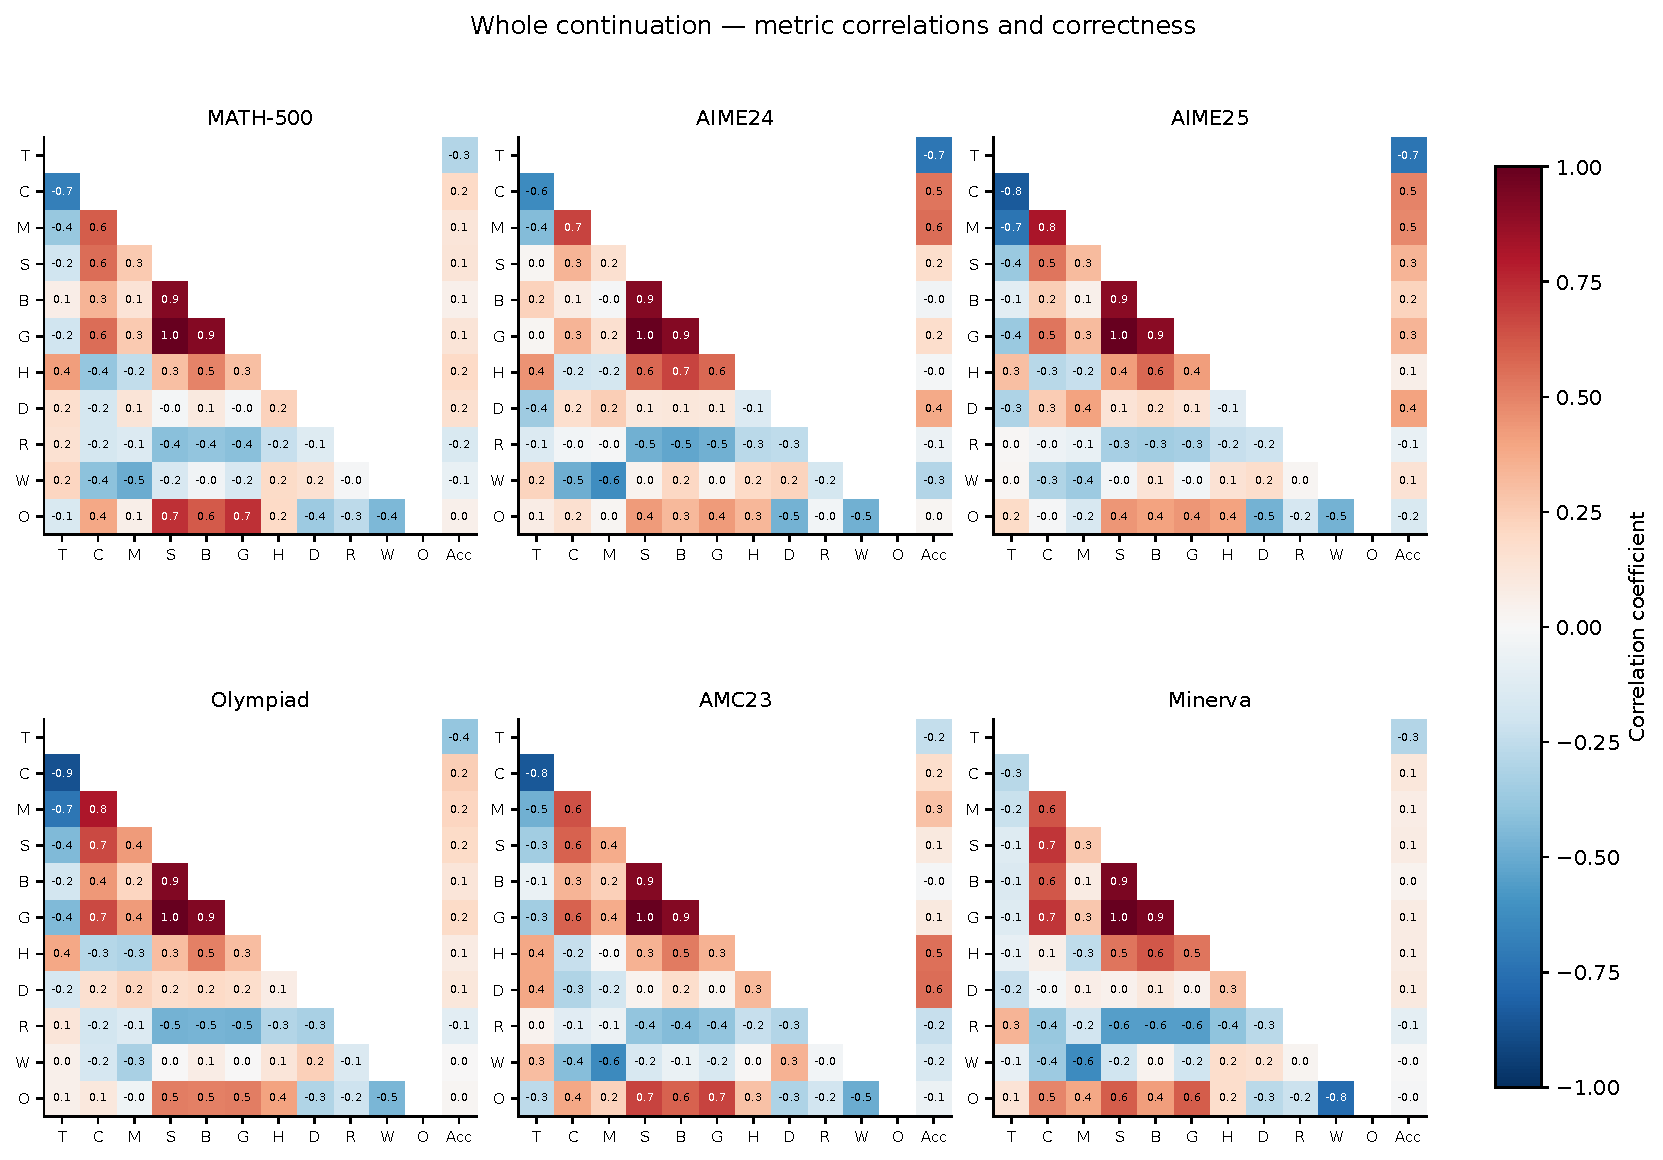
\includegraphics[width=\linewidth]{figures/qwen_atlas_continuation.pdf}
\caption{Whole continuation: metric relationships and correctness. Codes are defined in Table~\ref{tab:qwen-metric-key-atlas}.}
\label{fig:atlas-continuation}
\Description{Six benchmark heatmaps compare aggregate metrics with each other and with correctness.}
\end{figure}

\clearpage
\begin{figure}[p]
\centering
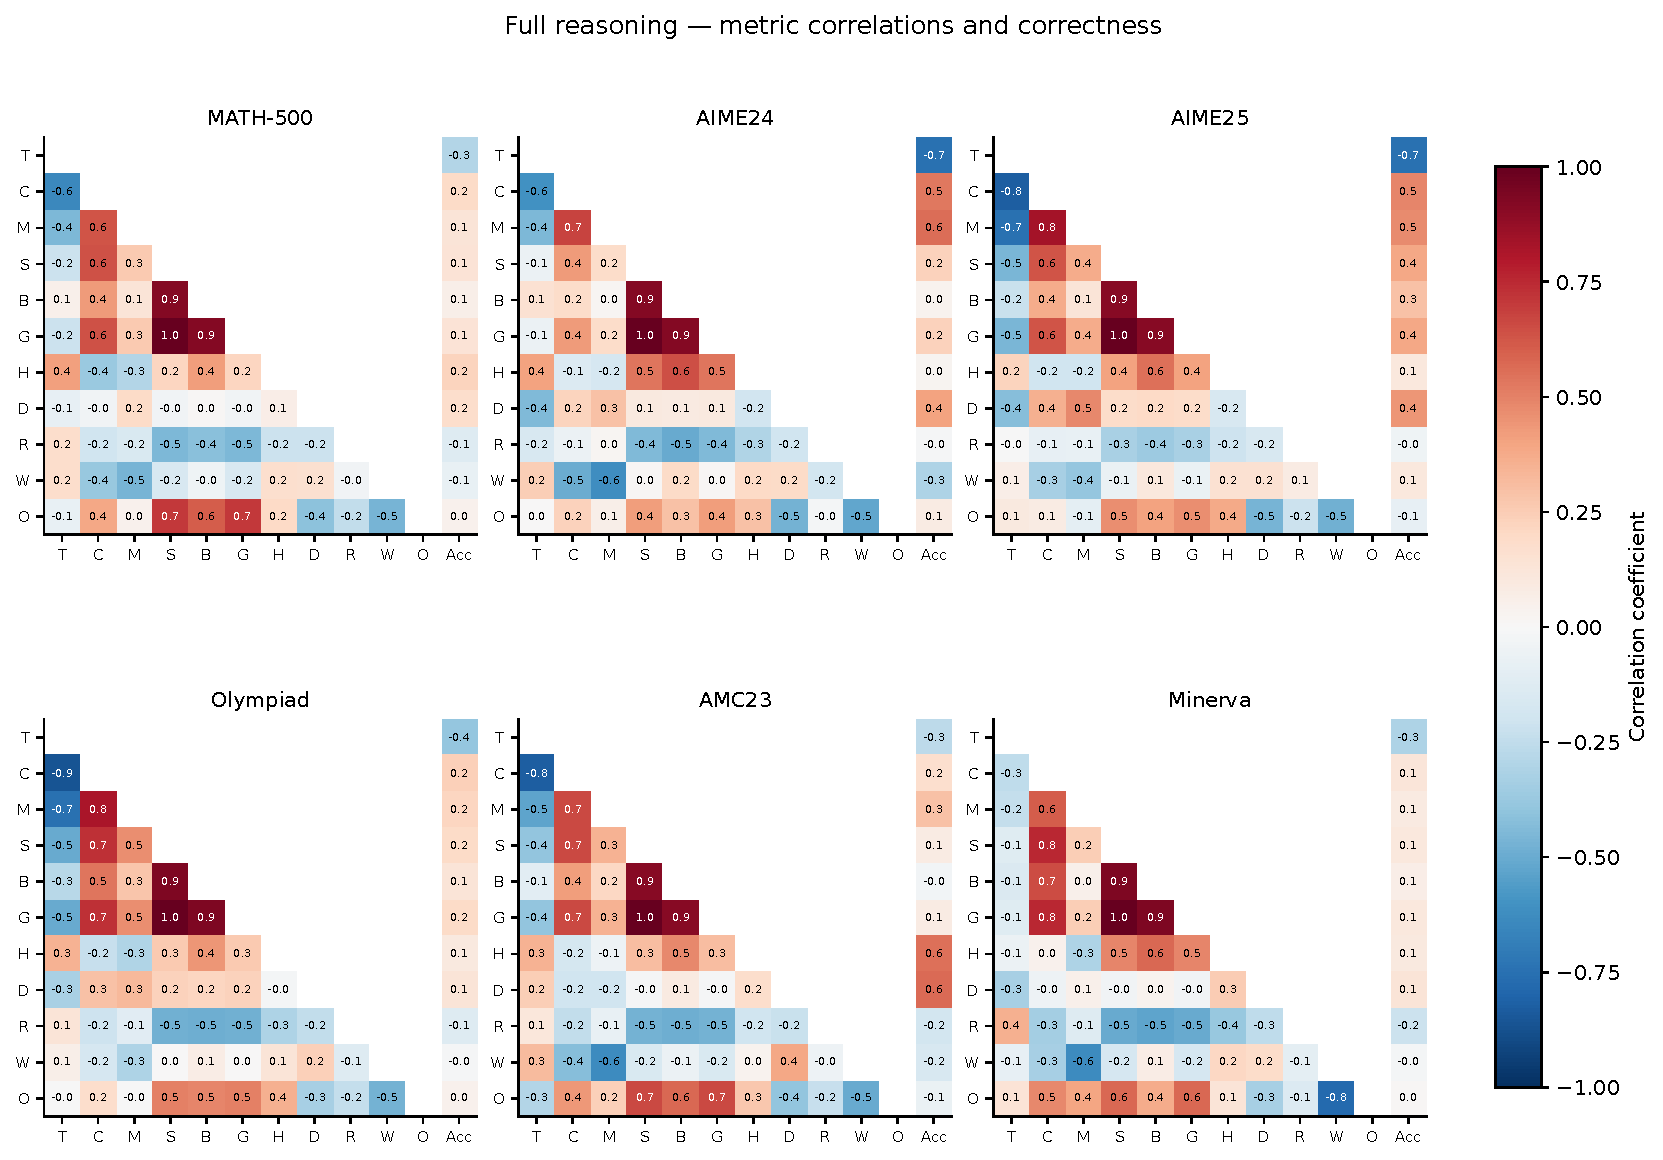
\includegraphics[width=\linewidth]{figures/qwen_atlas_reasoning.pdf}
\caption{Full reasoning: metric relationships and correctness. Codes are defined in Table~\ref{tab:qwen-metric-key-atlas}.}
\label{fig:atlas-reasoning}
\Description{Six benchmark heatmaps compare aggregate metrics with each other and with correctness.}
\end{figure}

\clearpage
\begin{figure}[p]
\centering
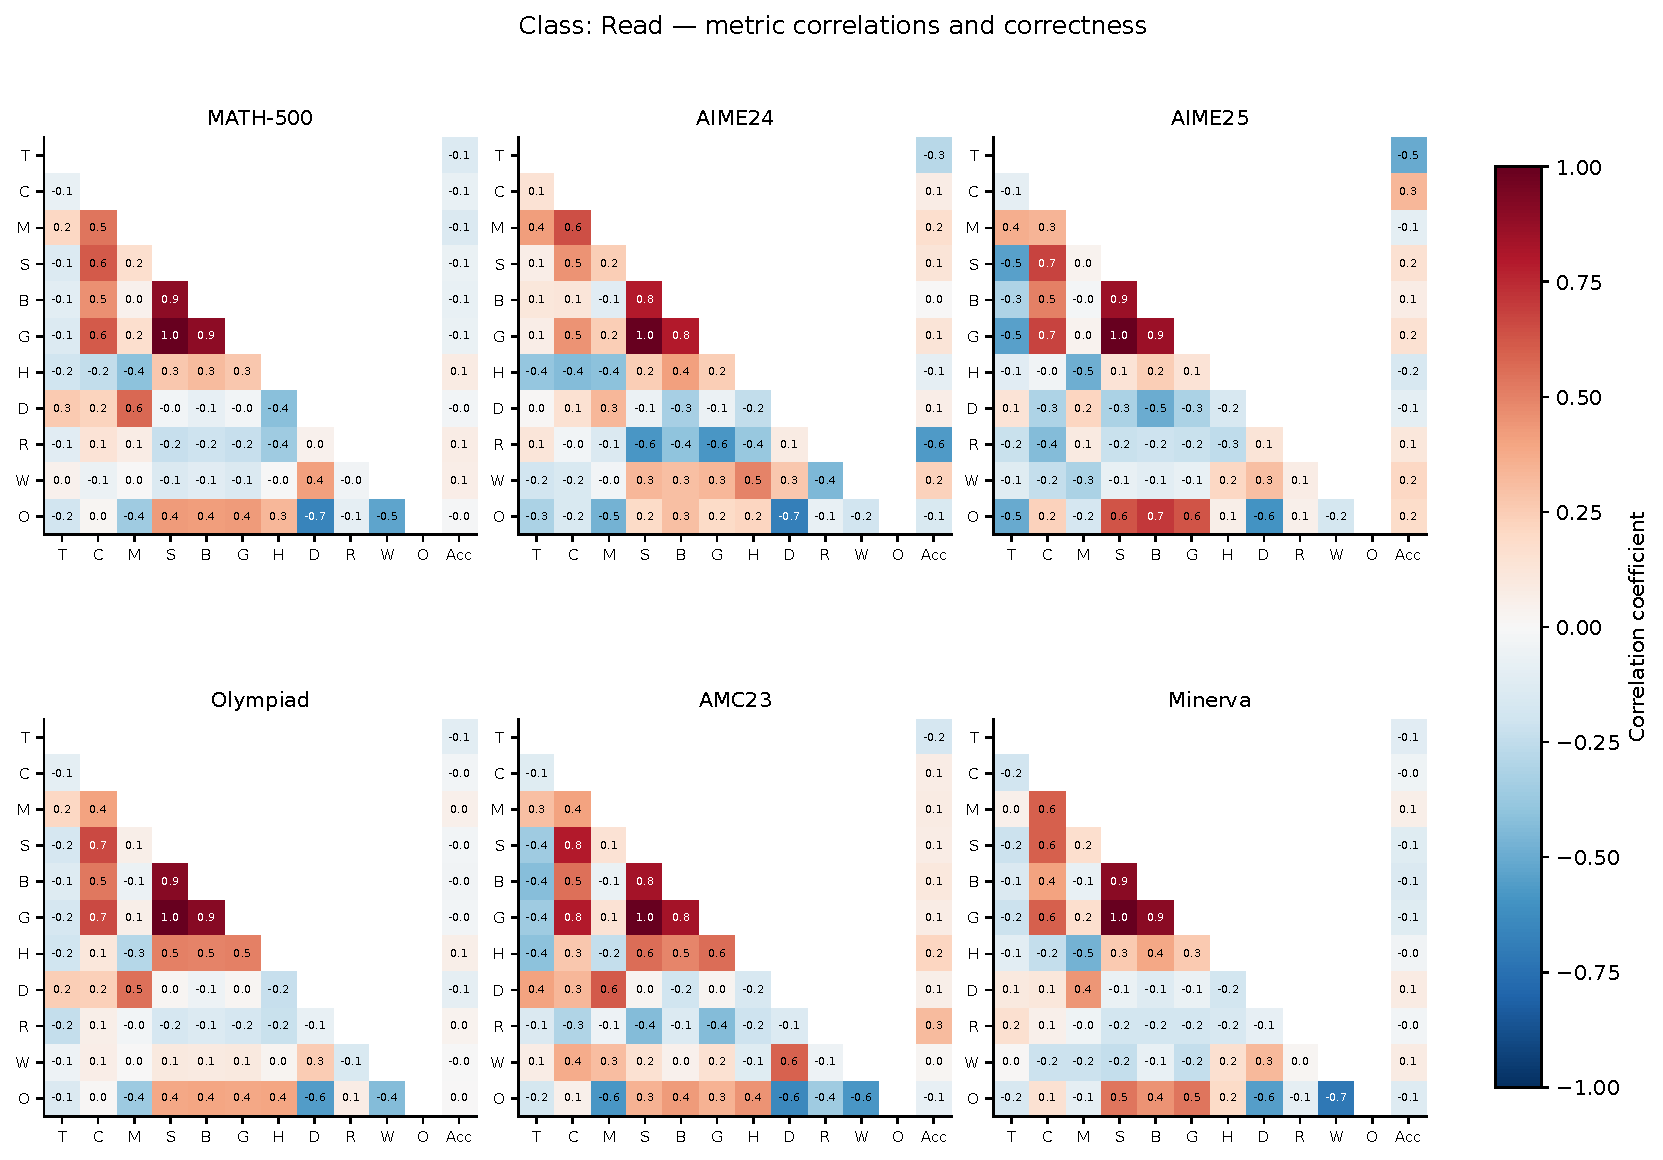
\includegraphics[width=\linewidth]{figures/qwen_atlas_class-Read.pdf}
\caption{Class: Read: metric relationships and correctness. Codes are defined in Table~\ref{tab:qwen-metric-key-atlas}.}
\label{fig:atlas-class-Read}
\Description{Six benchmark heatmaps compare aggregate metrics with each other and with correctness.}
\end{figure}

\clearpage
\begin{figure}[p]
\centering
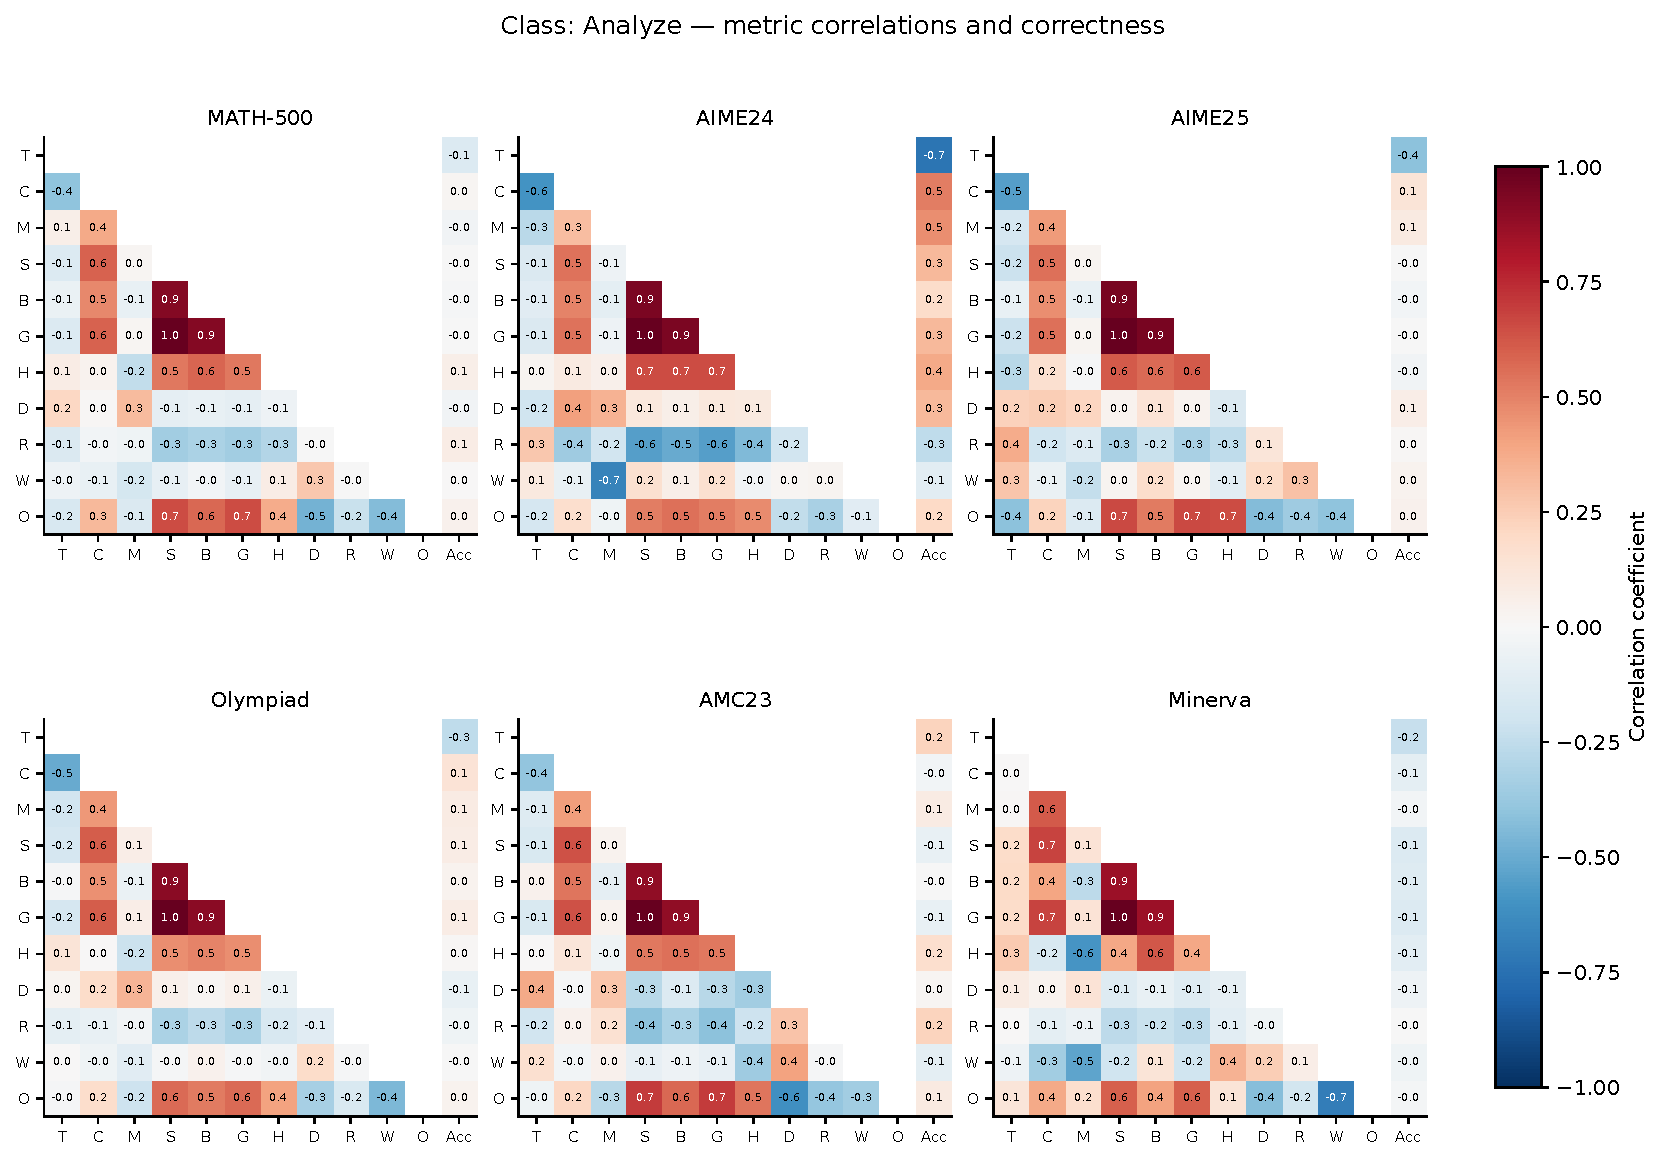
\includegraphics[width=\linewidth]{figures/qwen_atlas_class-Analyze.pdf}
\caption{Class: Analyze: metric relationships and correctness. Codes are defined in Table~\ref{tab:qwen-metric-key-atlas}.}
\label{fig:atlas-class-Analyze}
\Description{Six benchmark heatmaps compare aggregate metrics with each other and with correctness.}
\end{figure}

\clearpage
\begin{figure}[p]
\centering
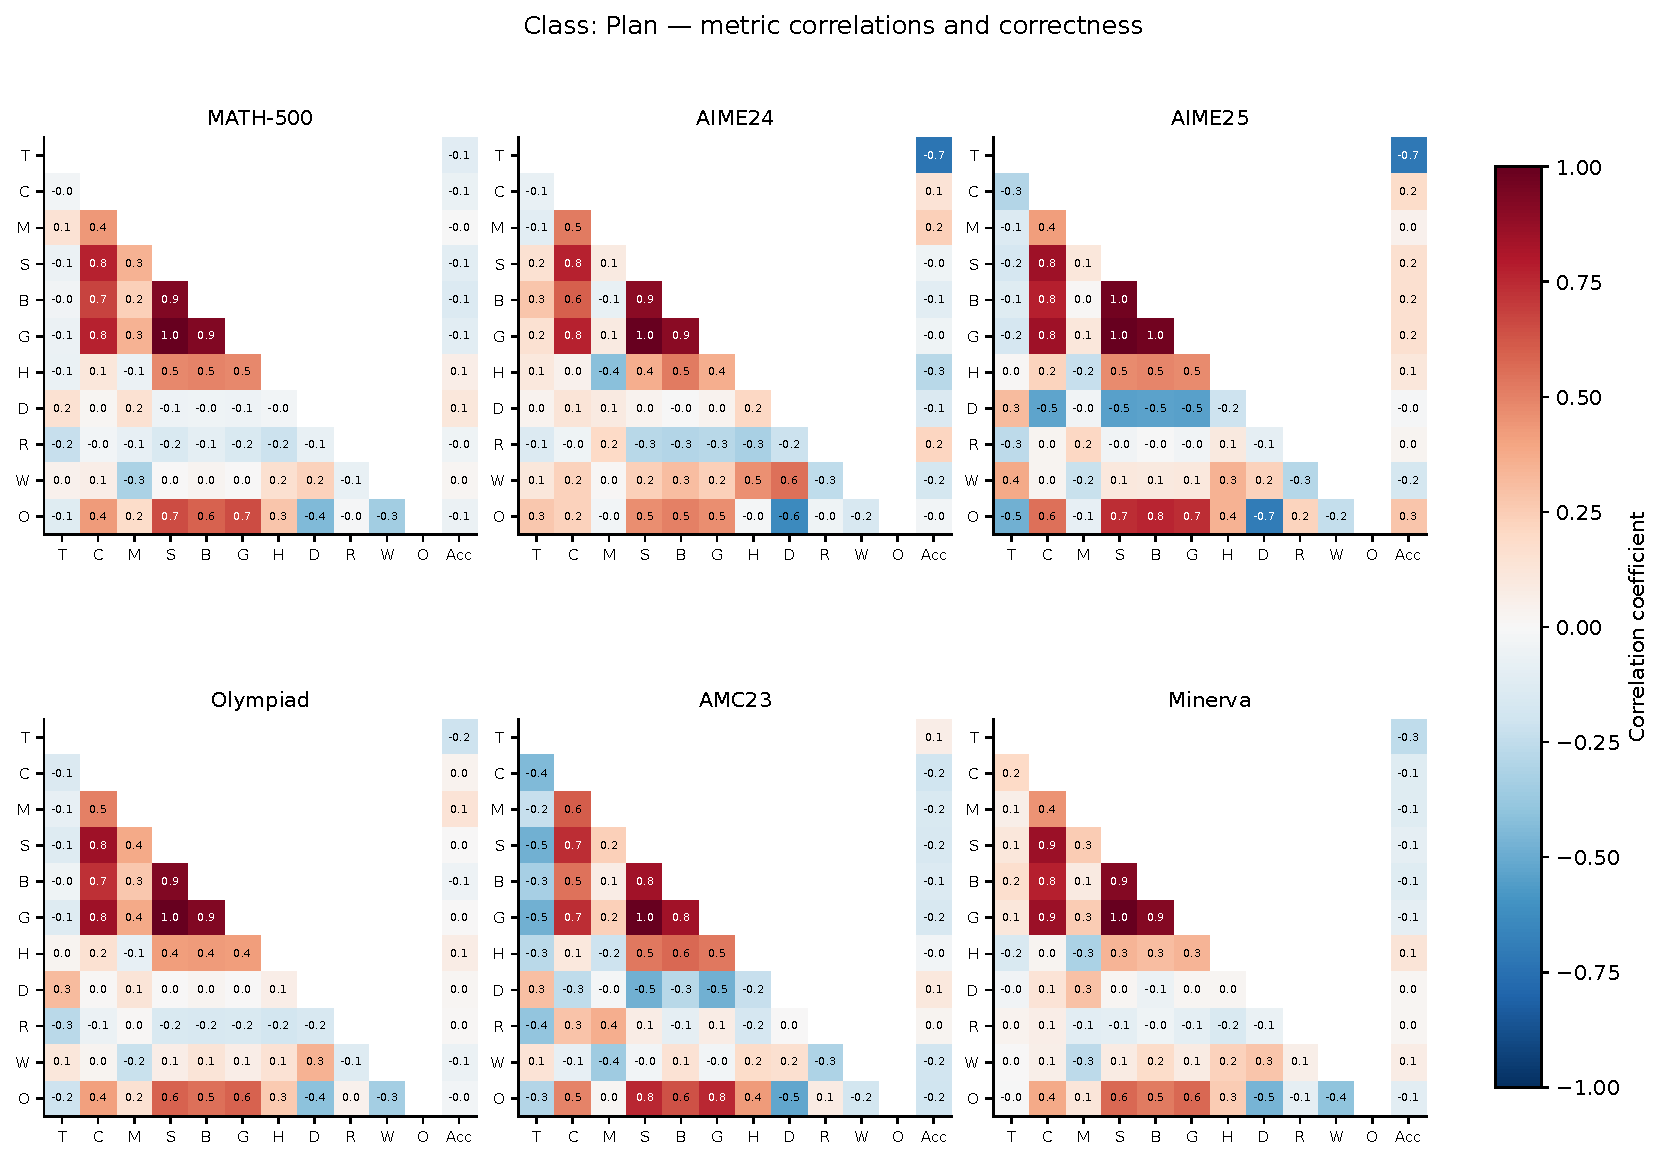
\includegraphics[width=\linewidth]{figures/qwen_atlas_class-Plan.pdf}
\caption{Class: Plan: metric relationships and correctness. Codes are defined in Table~\ref{tab:qwen-metric-key-atlas}.}
\label{fig:atlas-class-Plan}
\Description{Six benchmark heatmaps compare aggregate metrics with each other and with correctness.}
\end{figure}

\clearpage
\begin{figure}[p]
\centering
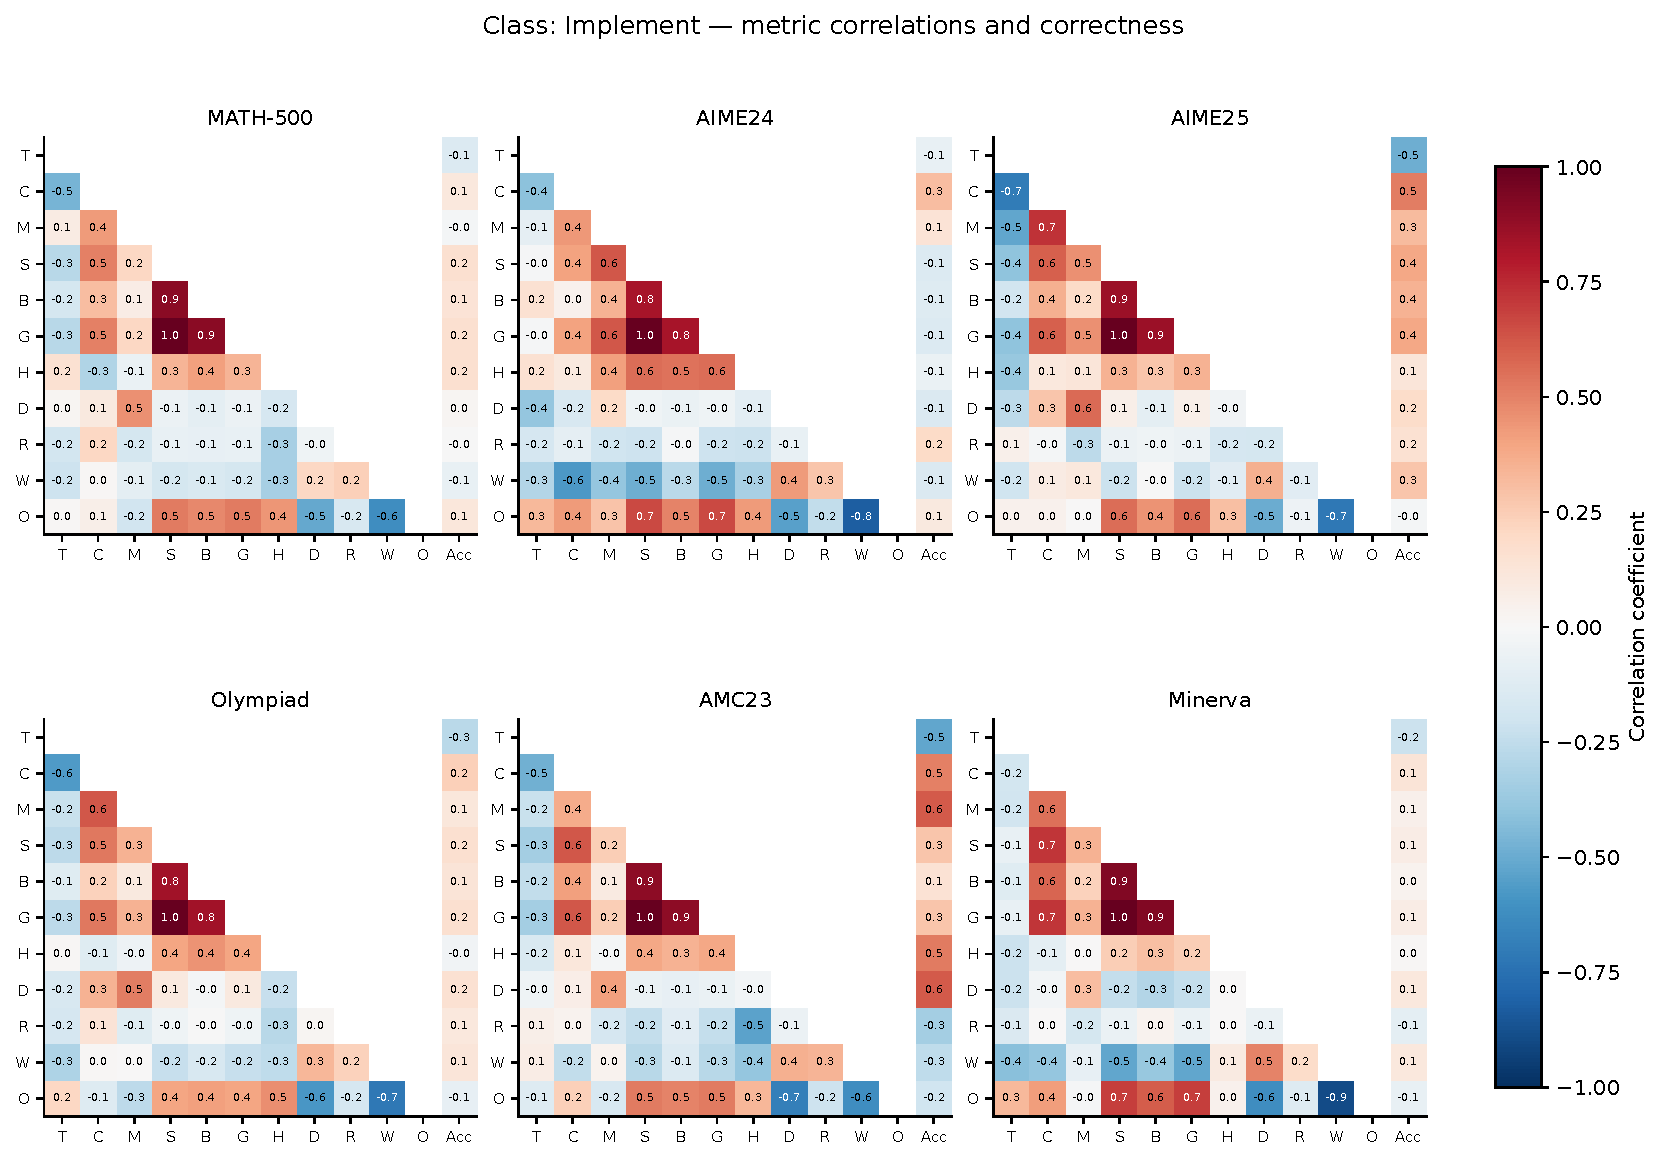
\includegraphics[width=\linewidth]{figures/qwen_atlas_class-Implement.pdf}
\caption{Class: Implement: metric relationships and correctness. Codes are defined in Table~\ref{tab:qwen-metric-key-atlas}.}
\label{fig:atlas-class-Implement}
\Description{Six benchmark heatmaps compare aggregate metrics with each other and with correctness.}
\end{figure}

\clearpage
\begin{figure}[p]
\centering
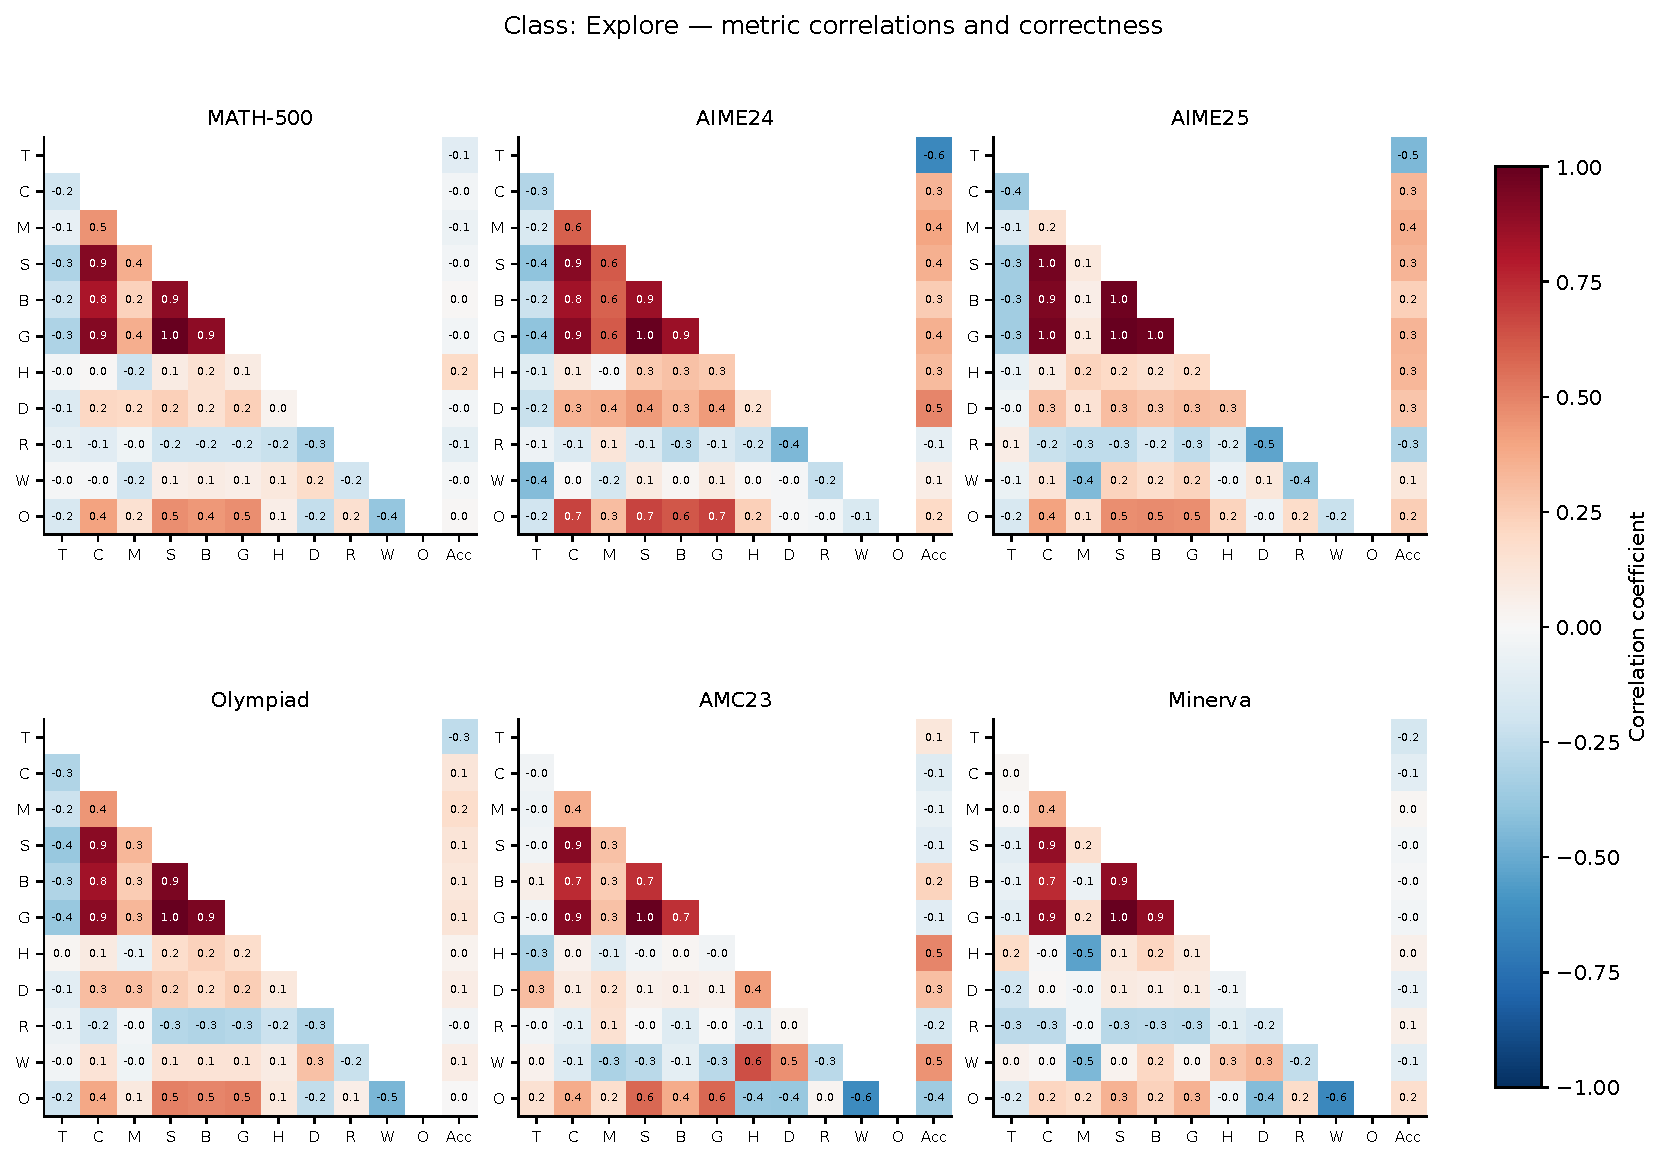
\includegraphics[width=\linewidth]{figures/qwen_atlas_class-Explore.pdf}
\caption{Class: Explore: metric relationships and correctness. Codes are defined in Table~\ref{tab:qwen-metric-key-atlas}.}
\label{fig:atlas-class-Explore}
\Description{Six benchmark heatmaps compare aggregate metrics with each other and with correctness.}
\end{figure}

\clearpage
\begin{figure}[p]
\centering
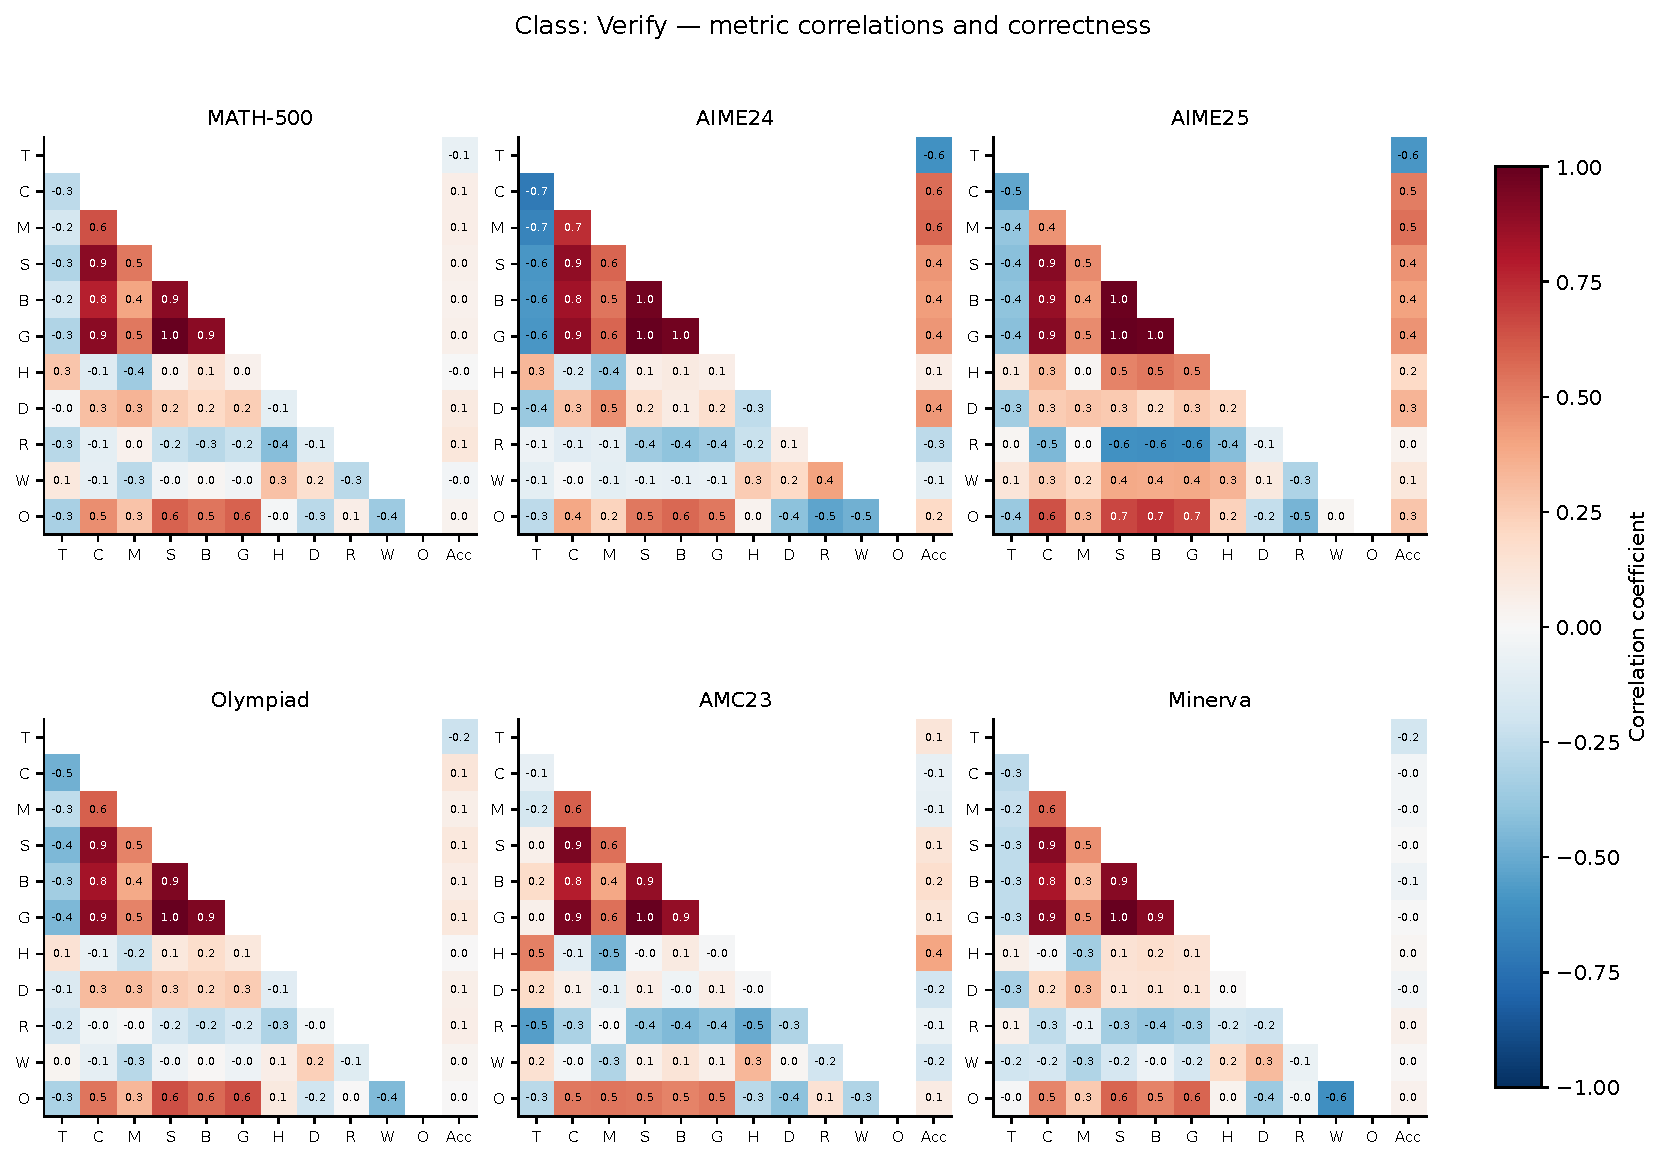
\includegraphics[width=\linewidth]{figures/qwen_atlas_class-Verify.pdf}
\caption{Class: Verify: metric relationships and correctness. Codes are defined in Table~\ref{tab:qwen-metric-key-atlas}.}
\label{fig:atlas-class-Verify}
\Description{Six benchmark heatmaps compare aggregate metrics with each other and with correctness.}
\end{figure}

\clearpage
\begin{figure}[p]
\centering
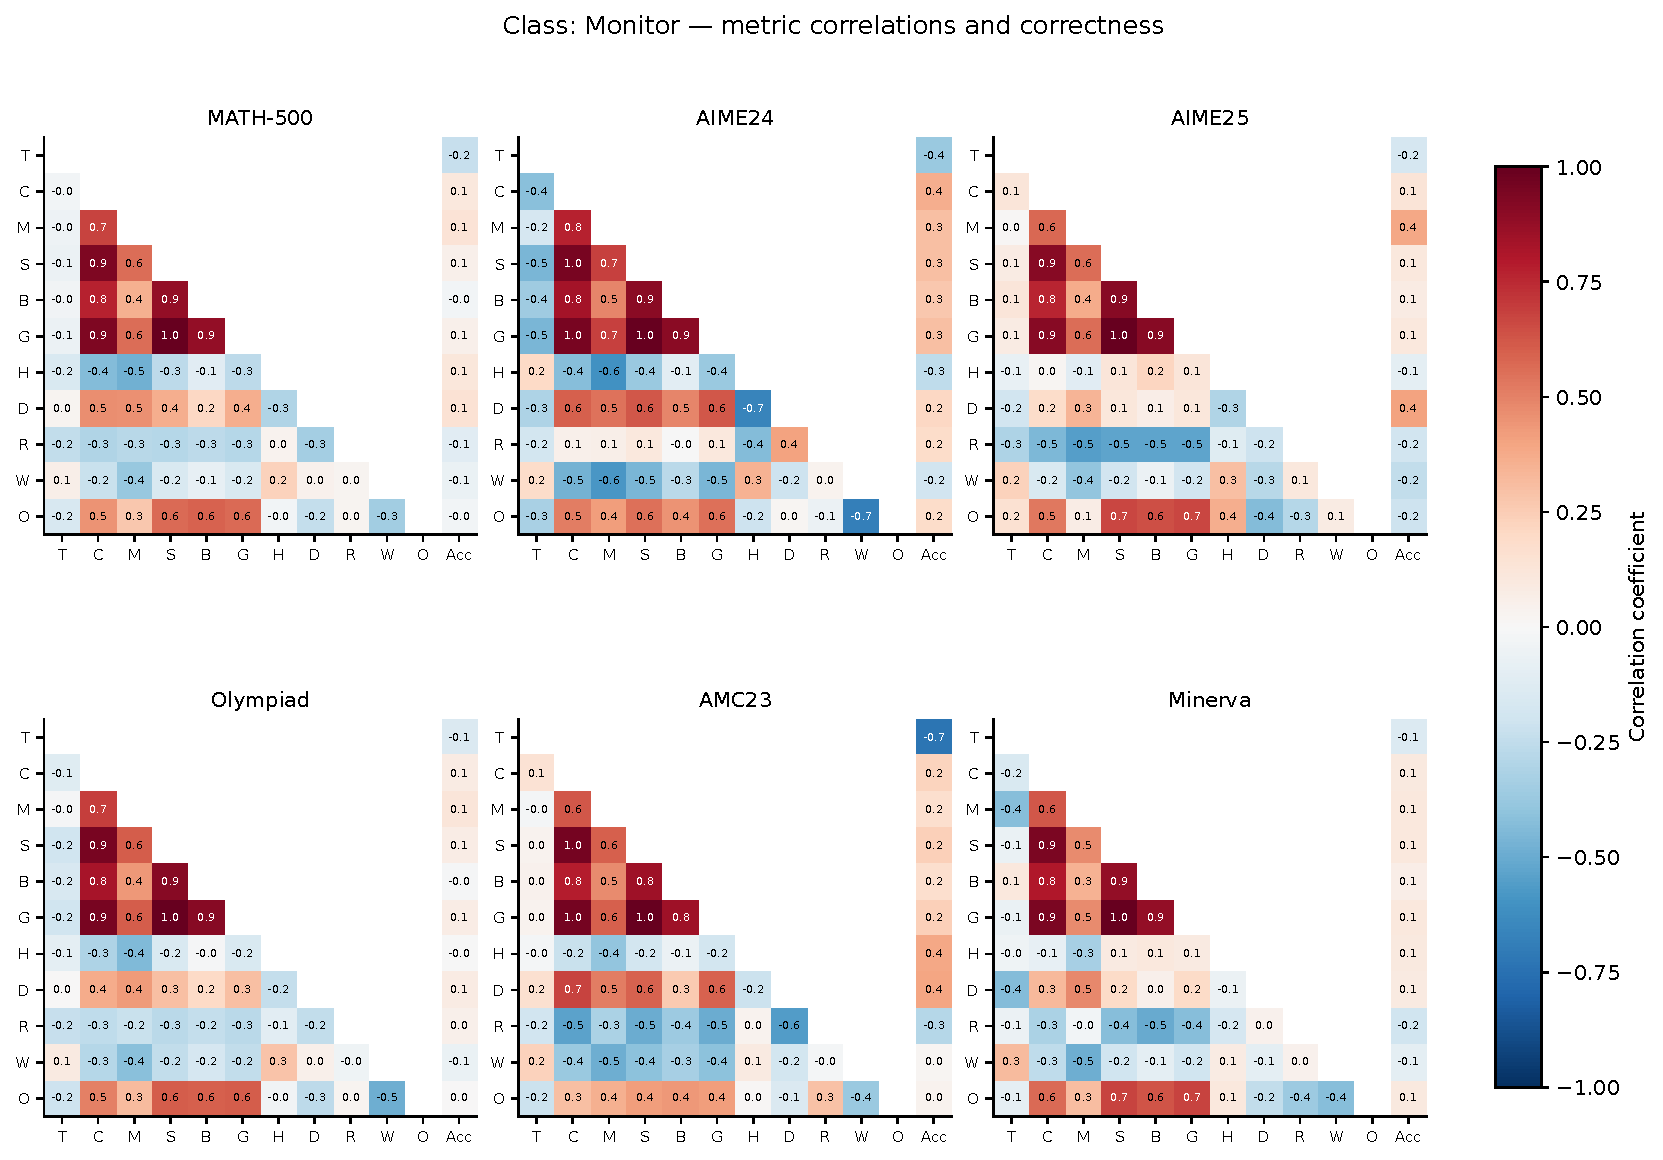
\includegraphics[width=\linewidth]{figures/qwen_atlas_class-Monitor.pdf}
\caption{Class: Monitor: metric relationships and correctness. Codes are defined in Table~\ref{tab:qwen-metric-key-atlas}.}
\label{fig:atlas-class-Monitor}
\Description{Six benchmark heatmaps compare aggregate metrics with each other and with correctness.}
\end{figure}

\clearpage
\begin{figure}[p]
\centering
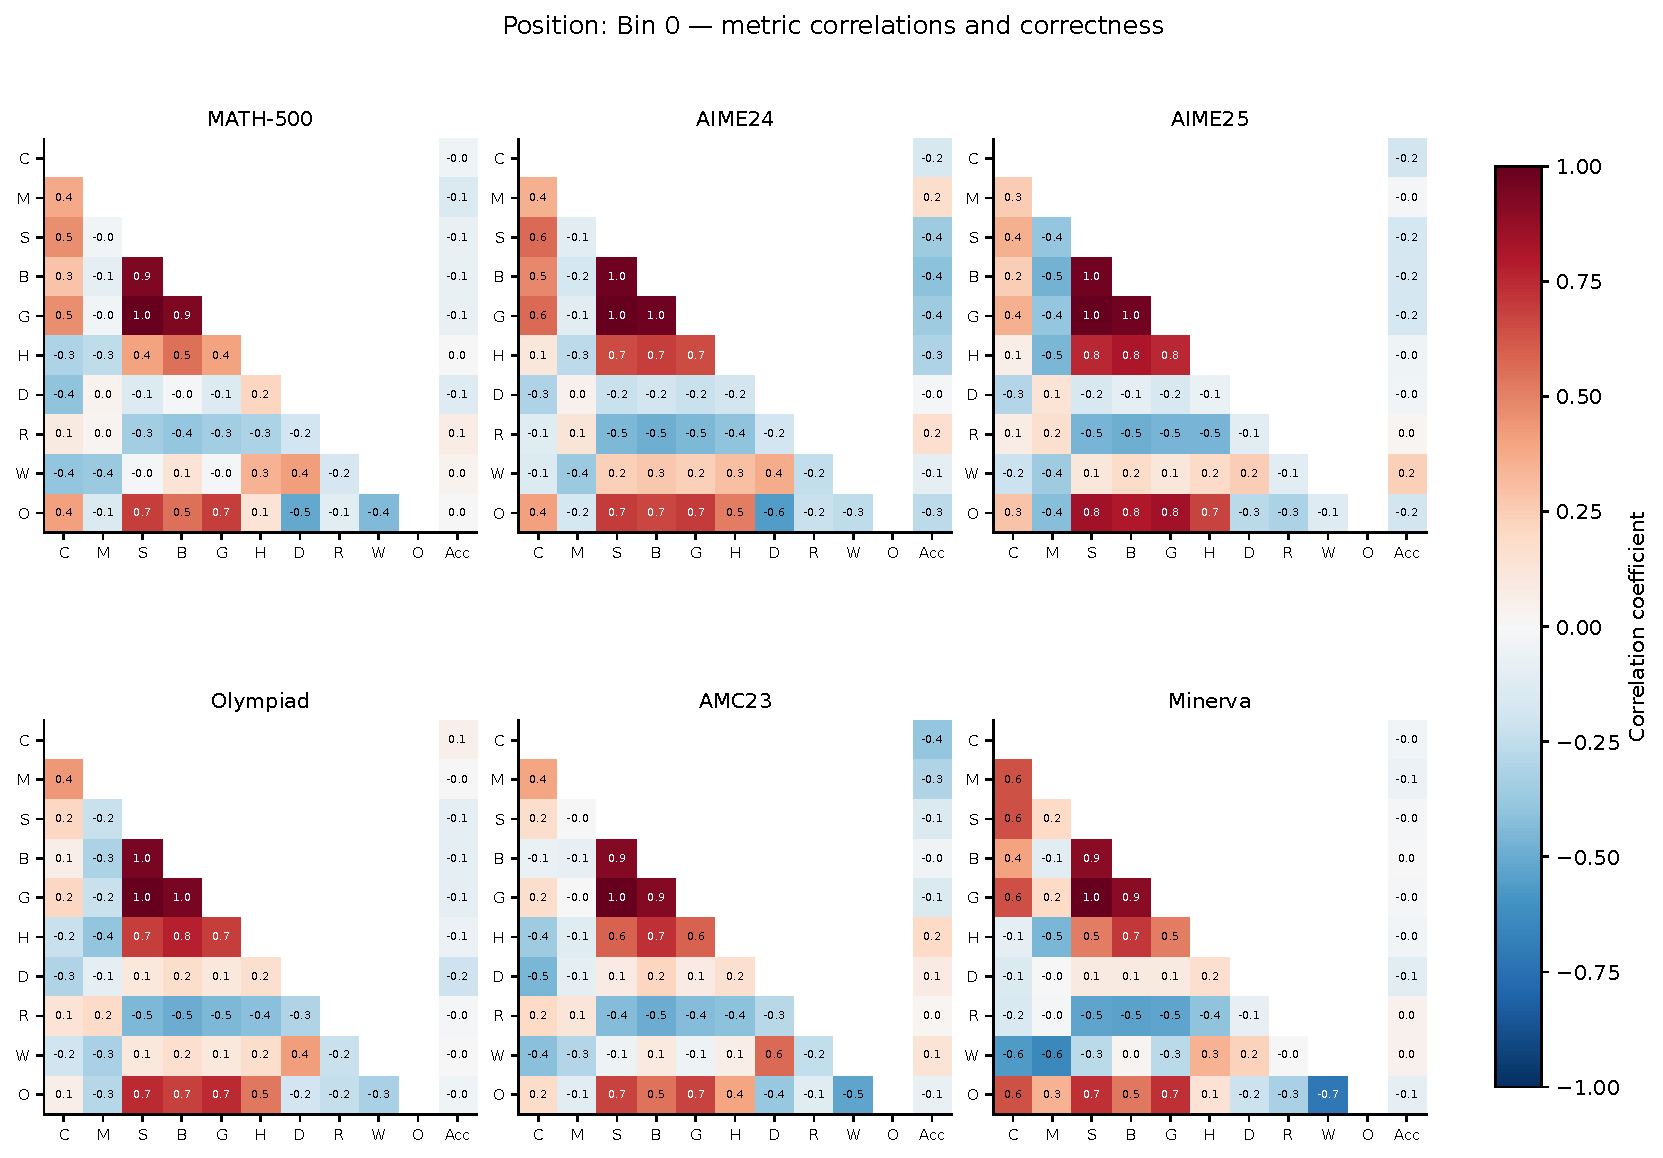
\includegraphics[width=\linewidth]{figures/qwen_atlas_position-bin-0.pdf}
\caption{Position: Bin 0: metric relationships and correctness. Codes are defined in Table~\ref{tab:qwen-metric-key-atlas}.}
\label{fig:atlas-position-bin-0}
\Description{Six benchmark heatmaps compare aggregate metrics with each other and with correctness.}
\end{figure}

\clearpage
\begin{figure}[p]
\centering
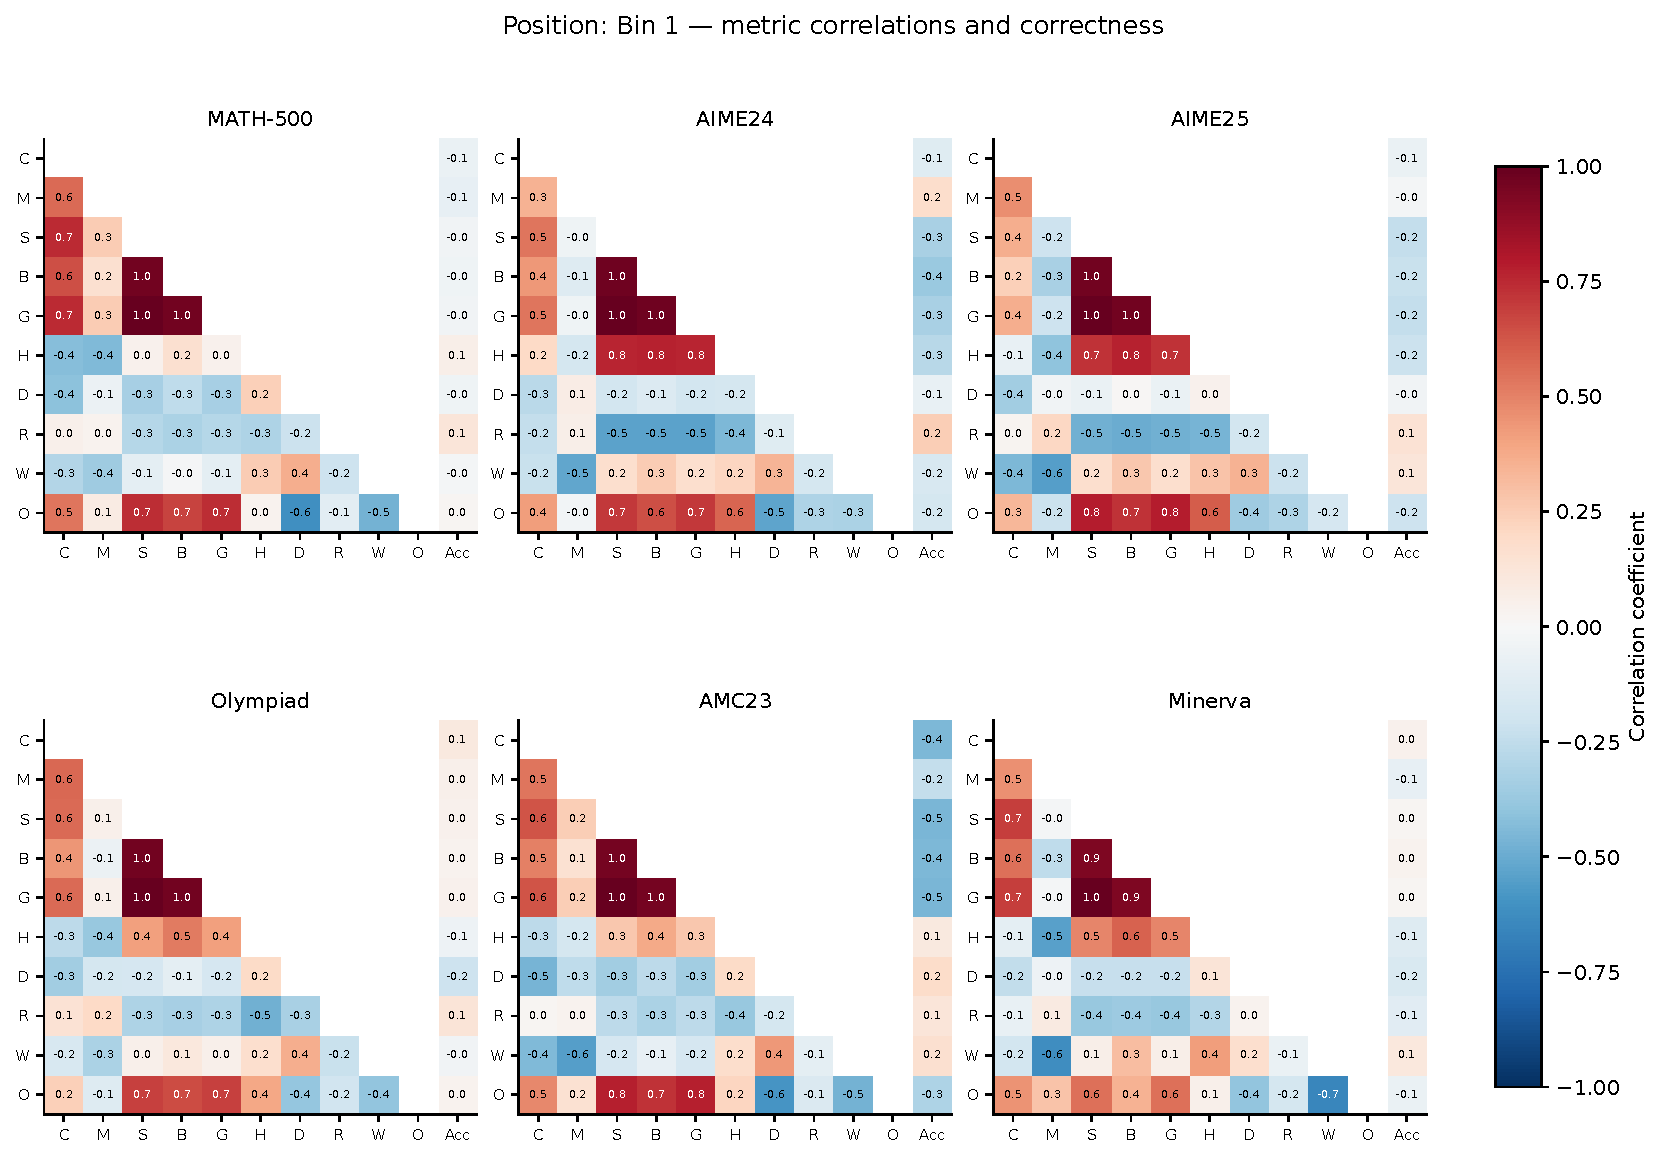
\includegraphics[width=\linewidth]{figures/qwen_atlas_position-bin-1.pdf}
\caption{Position: Bin 1: metric relationships and correctness. Codes are defined in Table~\ref{tab:qwen-metric-key-atlas}.}
\label{fig:atlas-position-bin-1}
\Description{Six benchmark heatmaps compare aggregate metrics with each other and with correctness.}
\end{figure}

\clearpage
\begin{figure}[p]
\centering
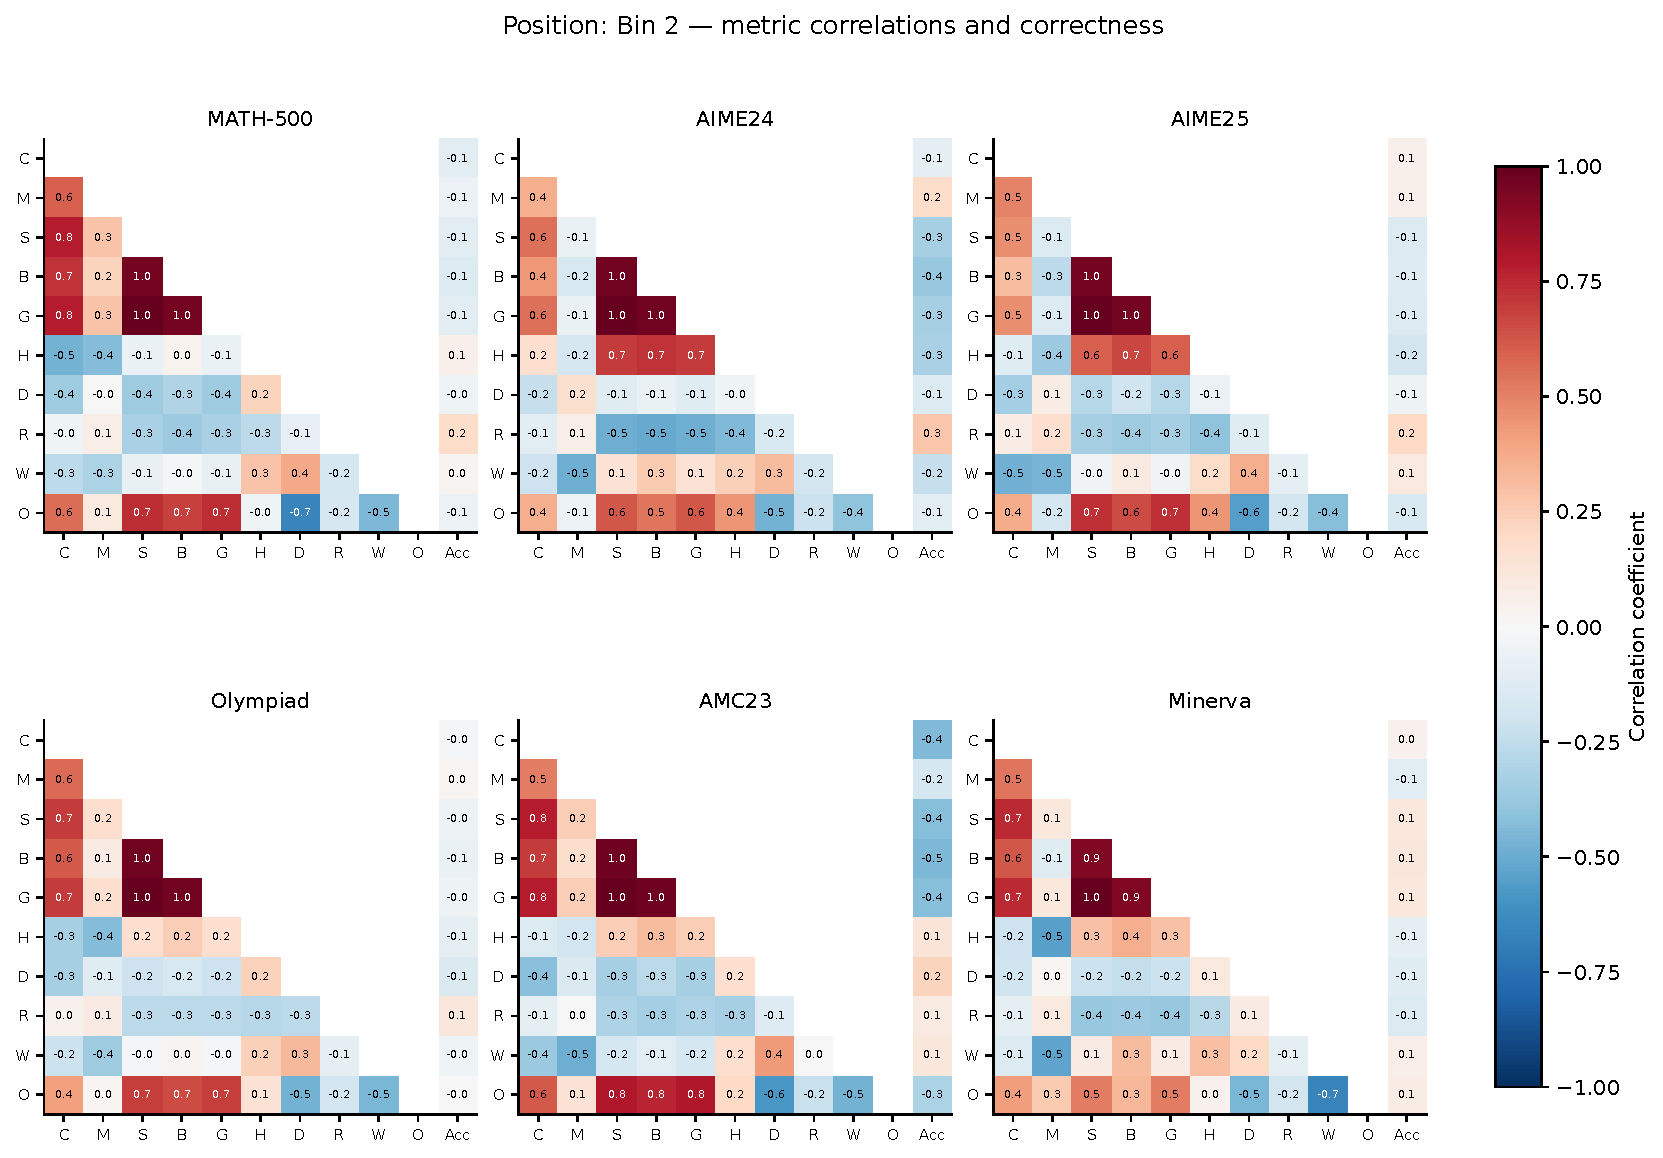
\includegraphics[width=\linewidth]{figures/qwen_atlas_position-bin-2.pdf}
\caption{Position: Bin 2: metric relationships and correctness. Codes are defined in Table~\ref{tab:qwen-metric-key-atlas}.}
\label{fig:atlas-position-bin-2}
\Description{Six benchmark heatmaps compare aggregate metrics with each other and with correctness.}
\end{figure}

\clearpage
\begin{figure}[p]
\centering
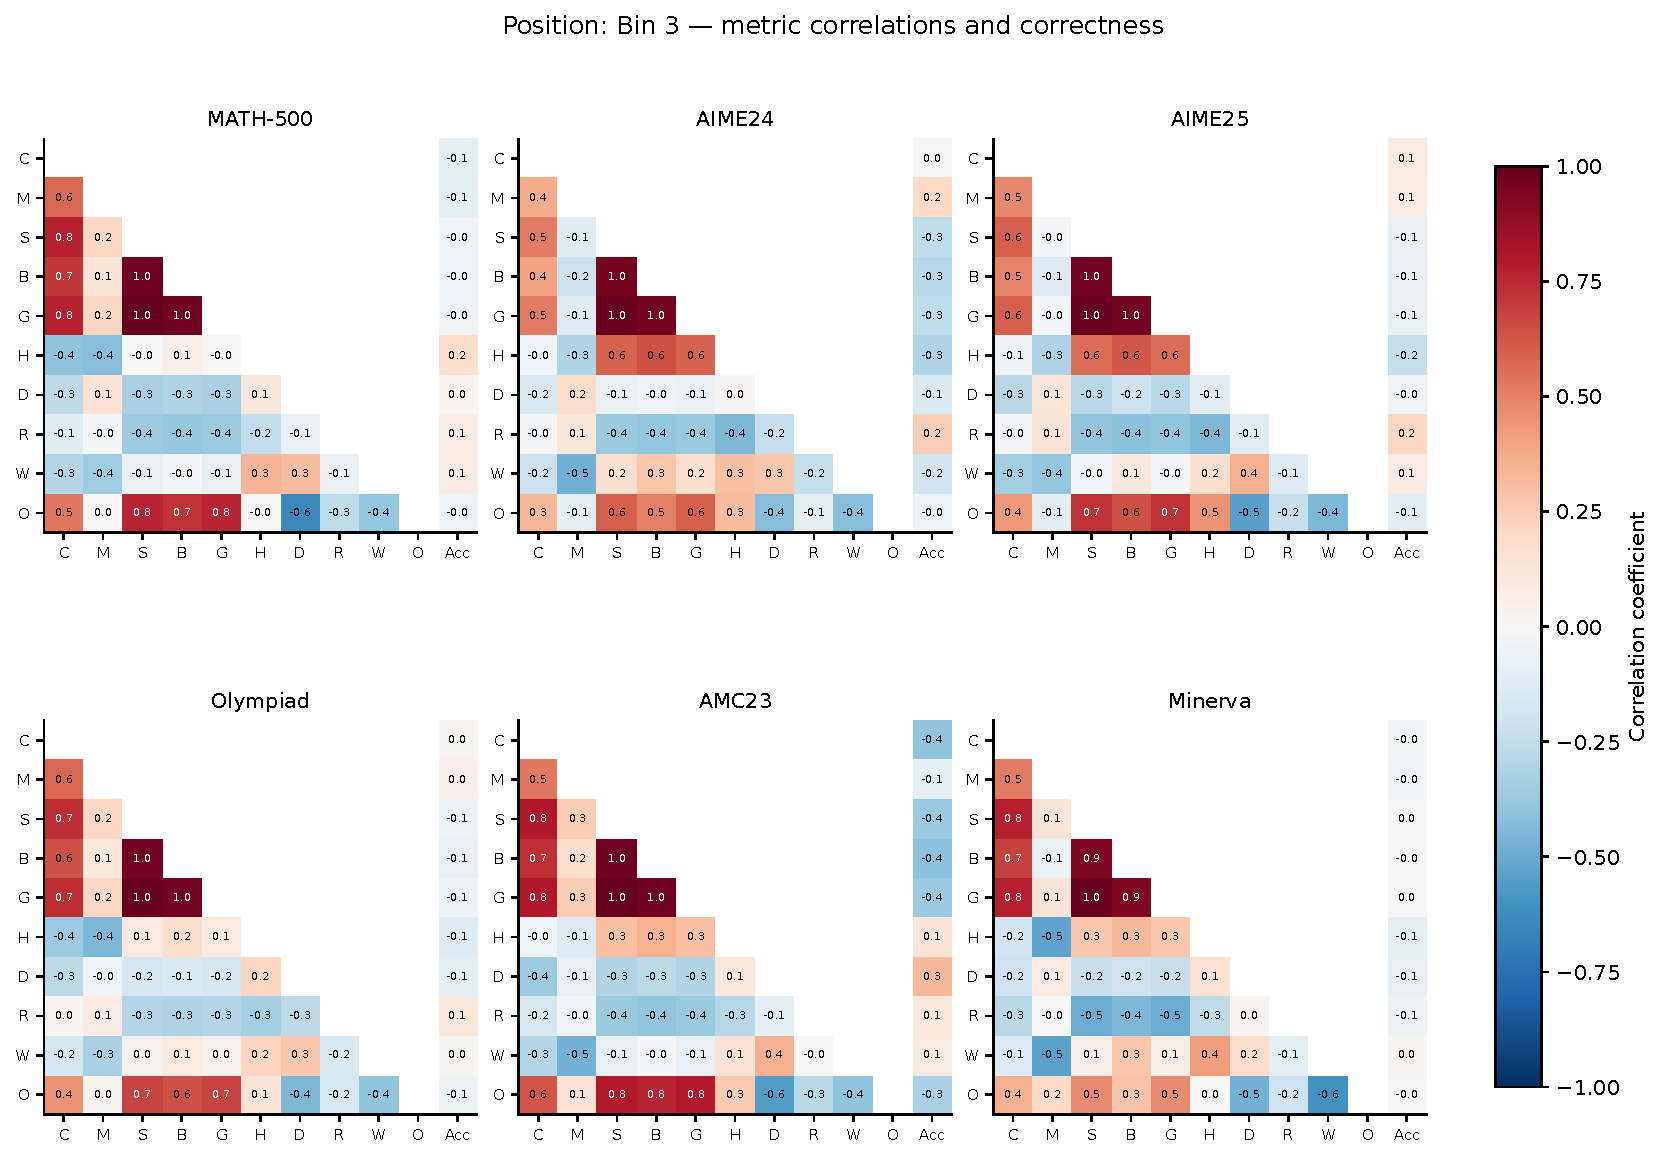
\includegraphics[width=\linewidth]{figures/qwen_atlas_position-bin-3.pdf}
\caption{Position: Bin 3: metric relationships and correctness. Codes are defined in Table~\ref{tab:qwen-metric-key-atlas}.}
\label{fig:atlas-position-bin-3}
\Description{Six benchmark heatmaps compare aggregate metrics with each other and with correctness.}
\end{figure}

\clearpage
\begin{figure}[p]
\centering
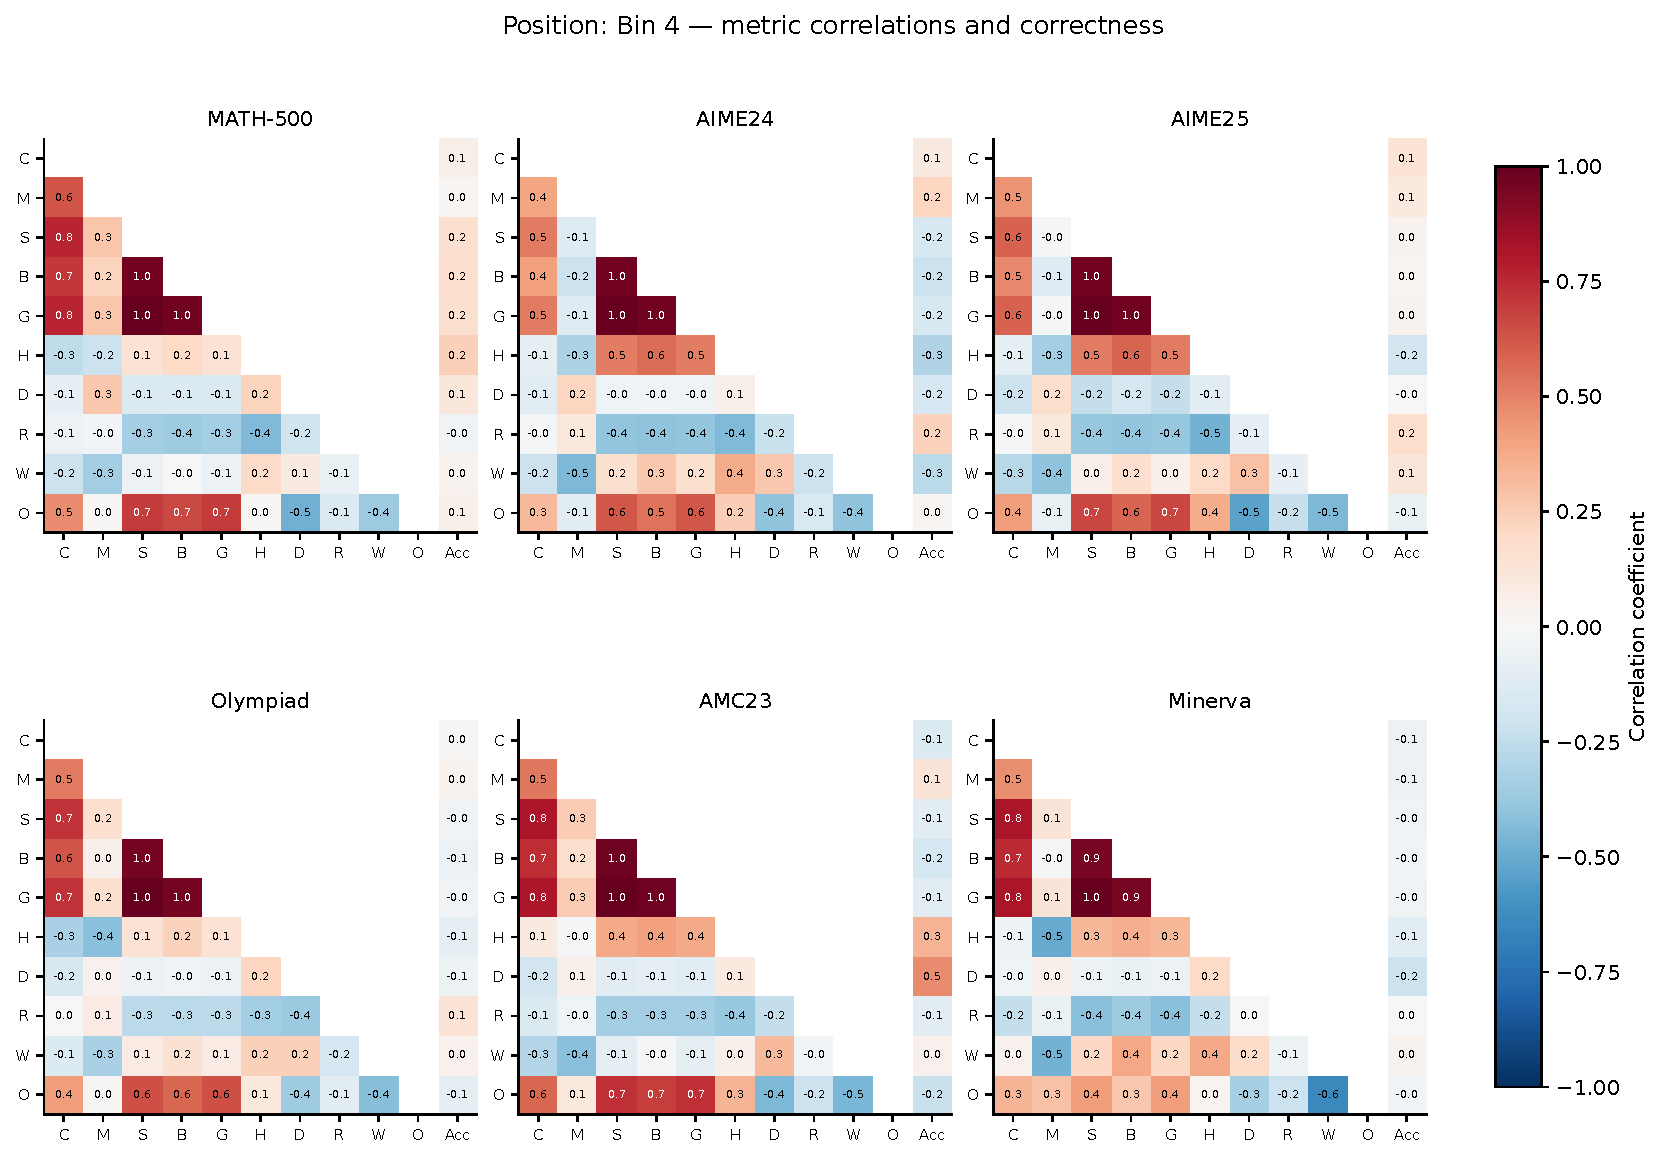
\includegraphics[width=\linewidth]{figures/qwen_atlas_position-bin-4.pdf}
\caption{Position: Bin 4: metric relationships and correctness. Codes are defined in Table~\ref{tab:qwen-metric-key-atlas}.}
\label{fig:atlas-position-bin-4}
\Description{Six benchmark heatmaps compare aggregate metrics with each other and with correctness.}
\end{figure}

\clearpage
\begin{figure}[p]
\centering
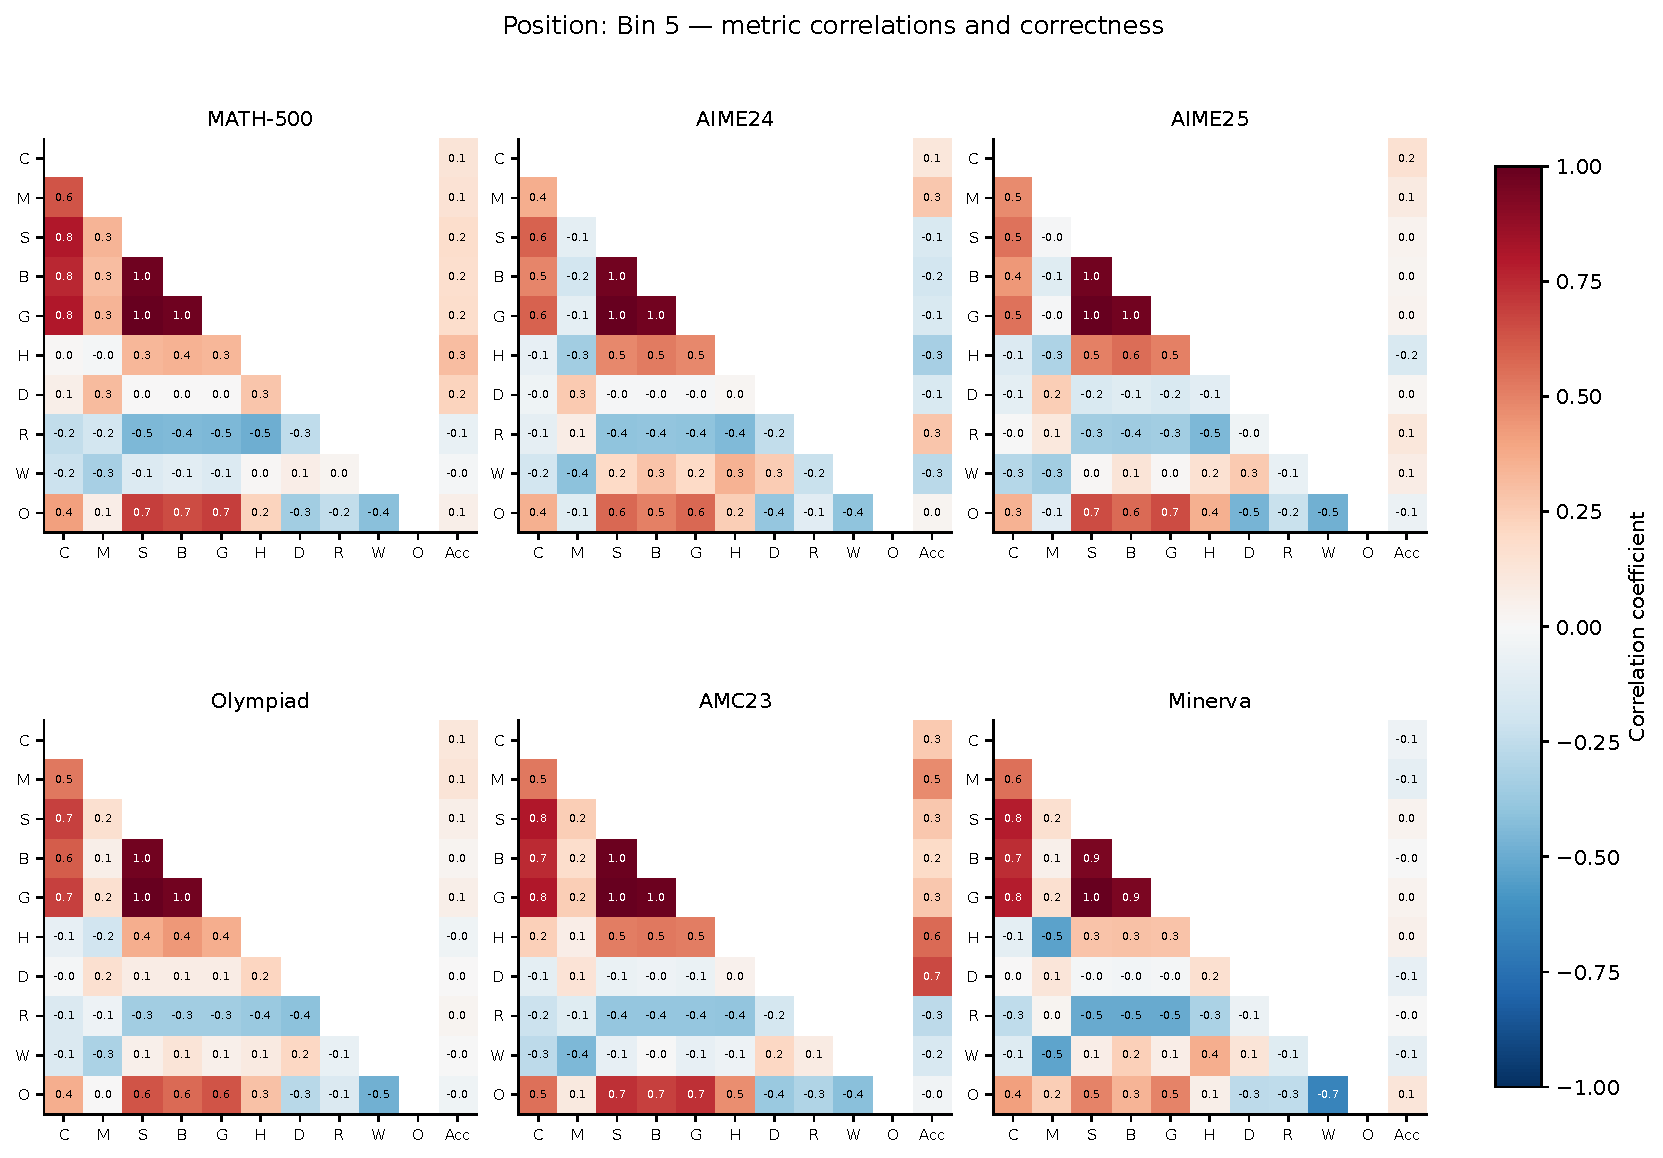
\includegraphics[width=\linewidth]{figures/qwen_atlas_position-bin-5.pdf}
\caption{Position: Bin 5: metric relationships and correctness. Codes are defined in Table~\ref{tab:qwen-metric-key-atlas}.}
\label{fig:atlas-position-bin-5}
\Description{Six benchmark heatmaps compare aggregate metrics with each other and with correctness.}
\end{figure}

\clearpage
\begin{figure}[p]
\centering
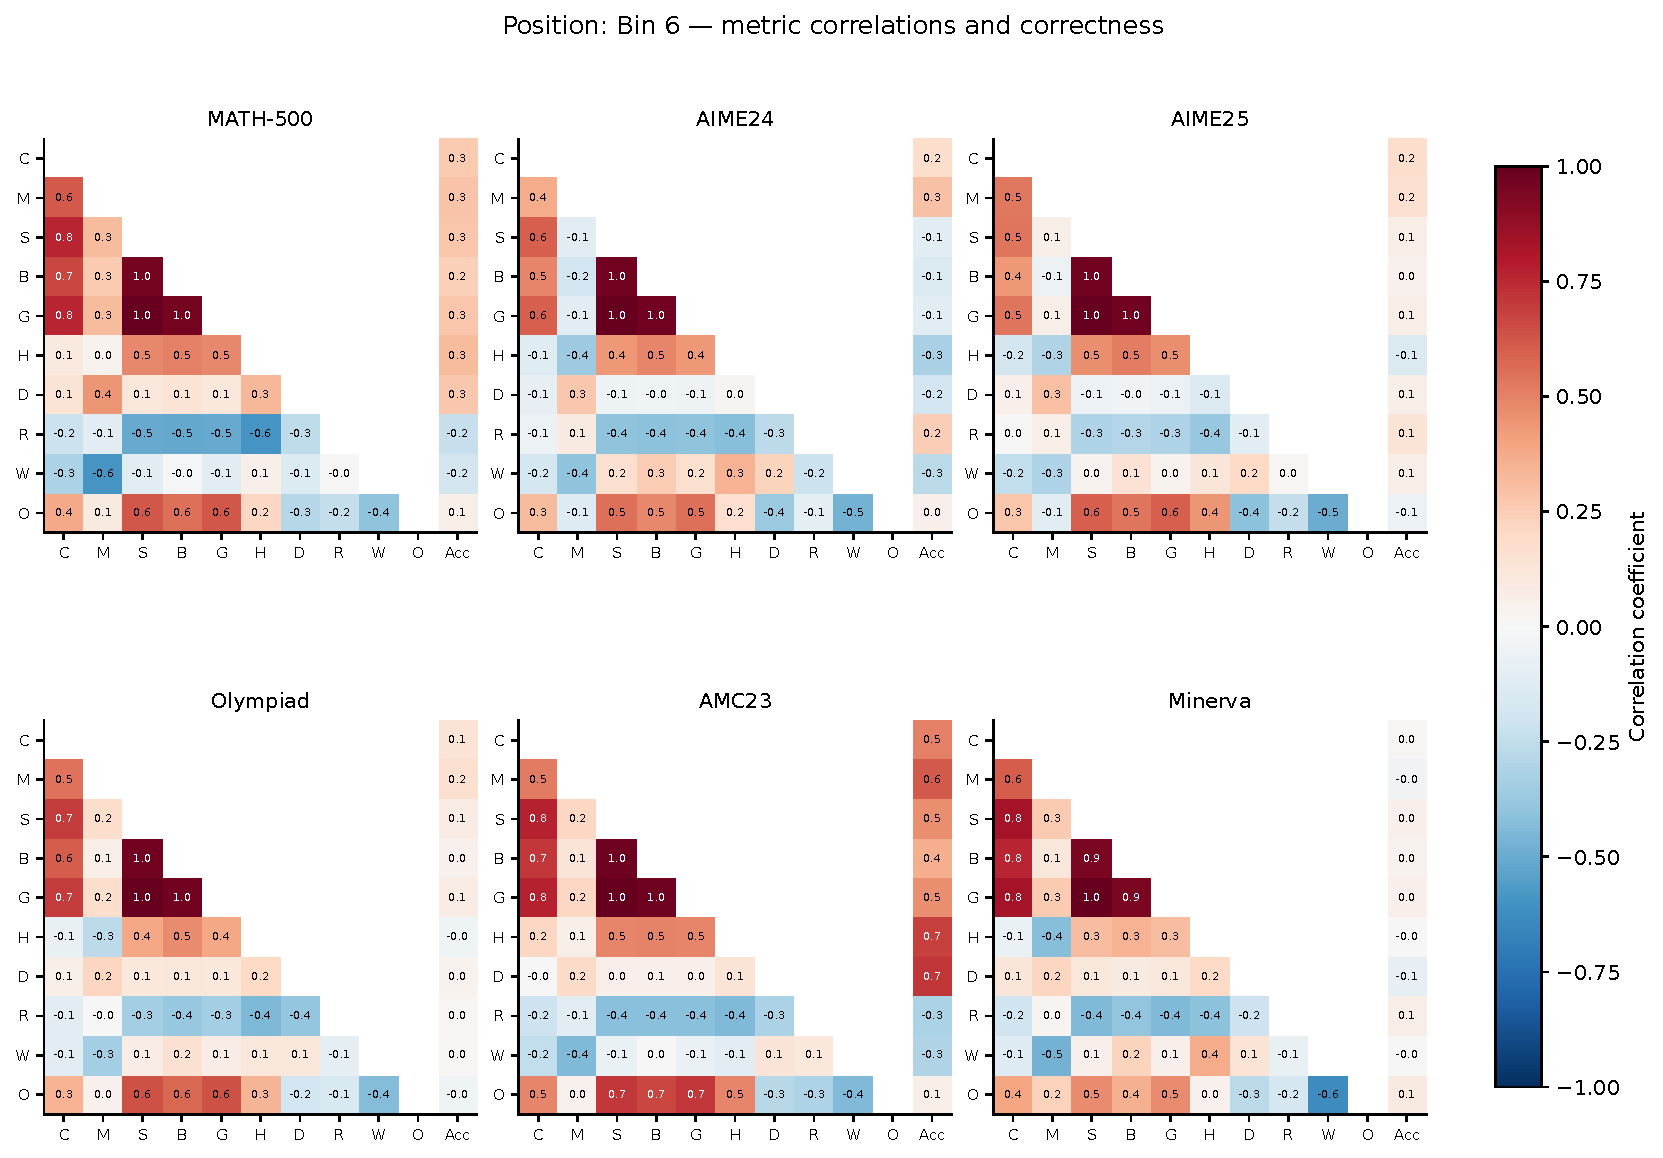
\includegraphics[width=\linewidth]{figures/qwen_atlas_position-bin-6.pdf}
\caption{Position: Bin 6: metric relationships and correctness. Codes are defined in Table~\ref{tab:qwen-metric-key-atlas}.}
\label{fig:atlas-position-bin-6}
\Description{Six benchmark heatmaps compare aggregate metrics with each other and with correctness.}
\end{figure}

\clearpage
\begin{figure}[p]
\centering
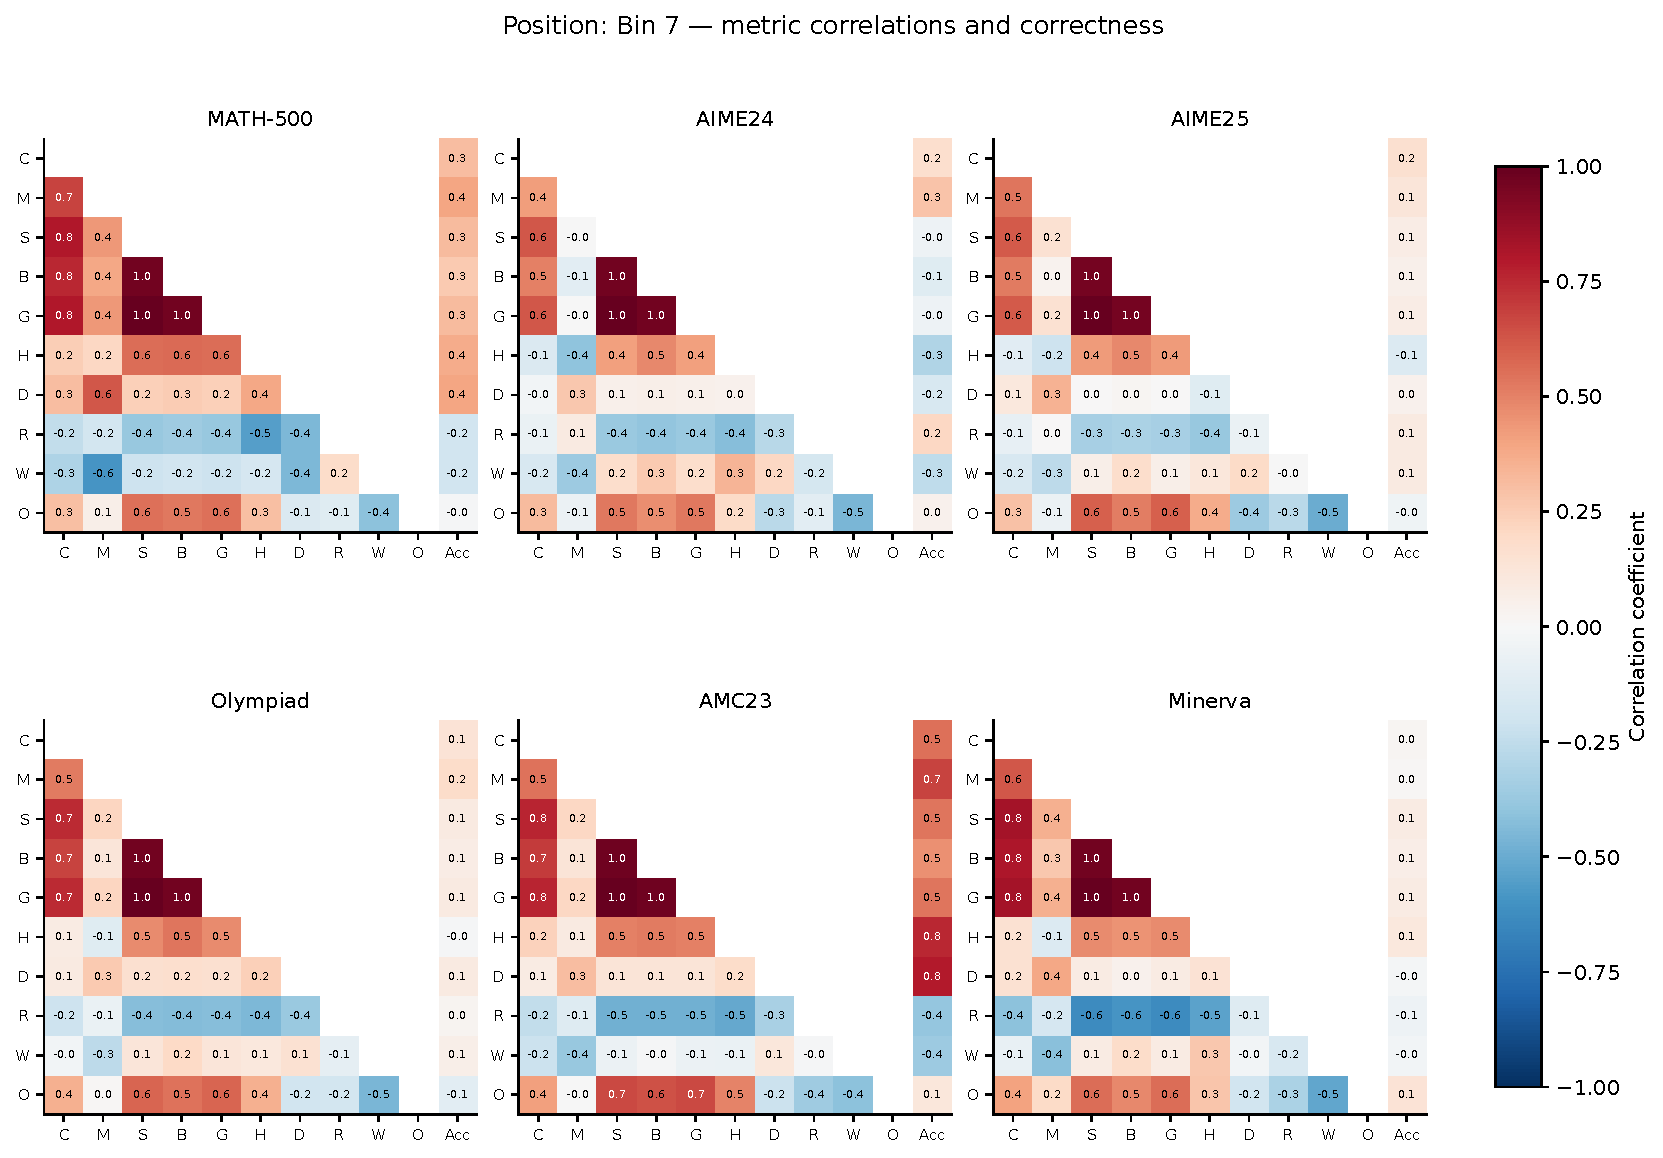
\includegraphics[width=\linewidth]{figures/qwen_atlas_position-bin-7.pdf}
\caption{Position: Bin 7: metric relationships and correctness. Codes are defined in Table~\ref{tab:qwen-metric-key-atlas}.}
\label{fig:atlas-position-bin-7}
\Description{Six benchmark heatmaps compare aggregate metrics with each other and with correctness.}
\end{figure}

\clearpage
\begin{figure}[p]
\centering
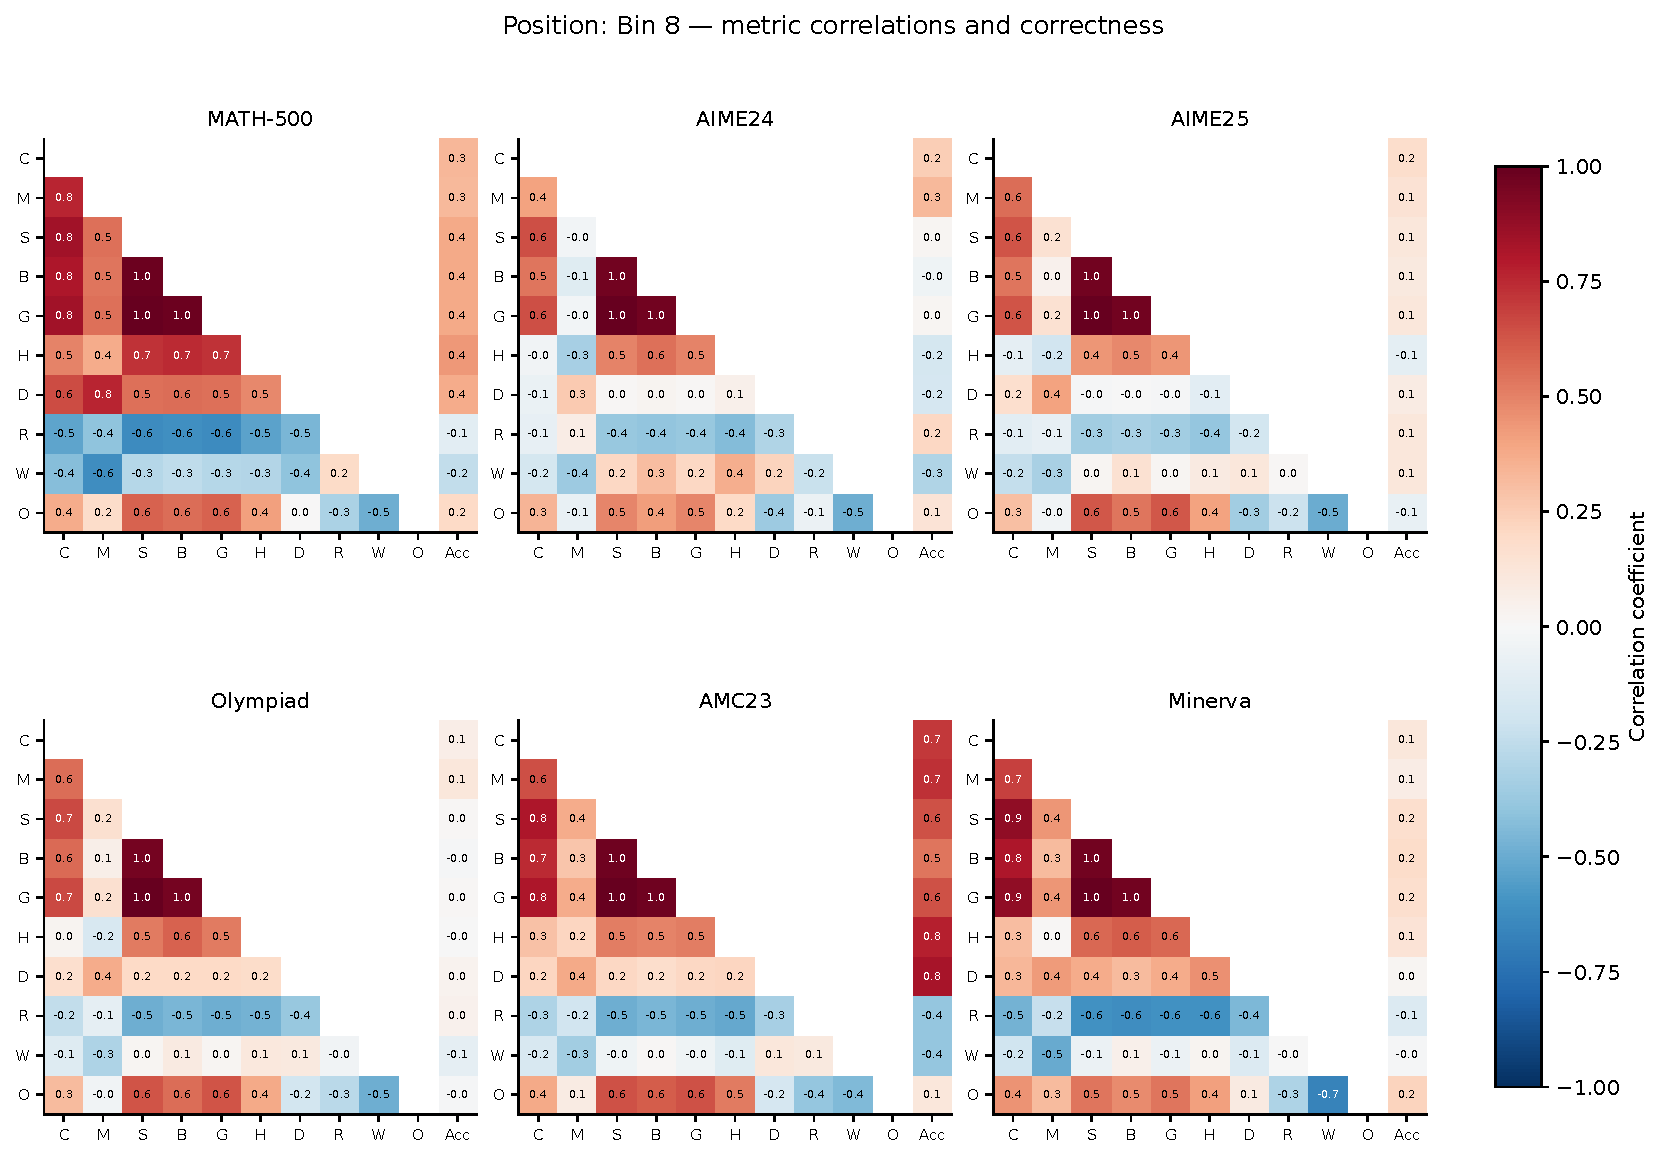
\includegraphics[width=\linewidth]{figures/qwen_atlas_position-bin-8.pdf}
\caption{Position: Bin 8: metric relationships and correctness. Codes are defined in Table~\ref{tab:qwen-metric-key-atlas}.}
\label{fig:atlas-position-bin-8}
\Description{Six benchmark heatmaps compare aggregate metrics with each other and with correctness.}
\end{figure}

\clearpage
\begin{figure}[p]
\centering
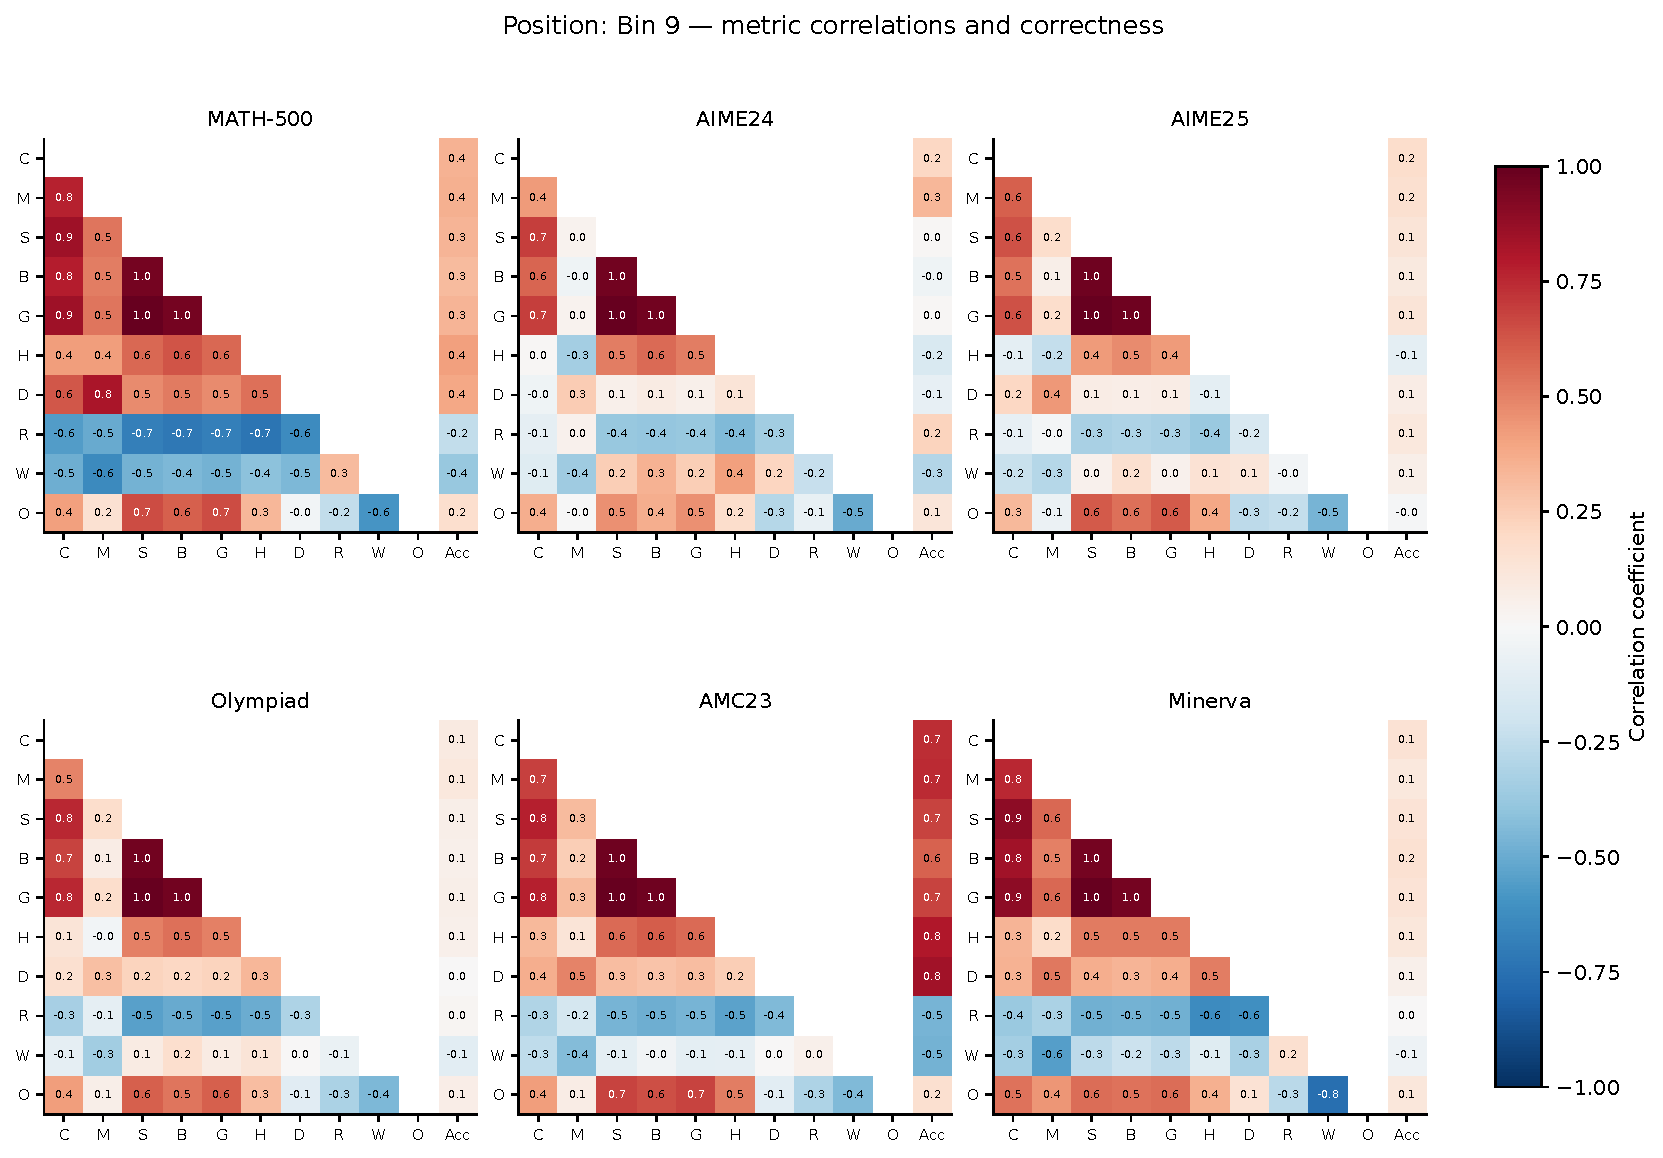
\includegraphics[width=\linewidth]{figures/qwen_atlas_position-bin-9.pdf}
\caption{Position: Bin 9: metric relationships and correctness. Codes are defined in Table~\ref{tab:qwen-metric-key-atlas}.}
\label{fig:atlas-position-bin-9}
\Description{Six benchmark heatmaps compare aggregate metrics with each other and with correctness.}
\end{figure}

\clearpage
\begin{figure}[p]
\centering
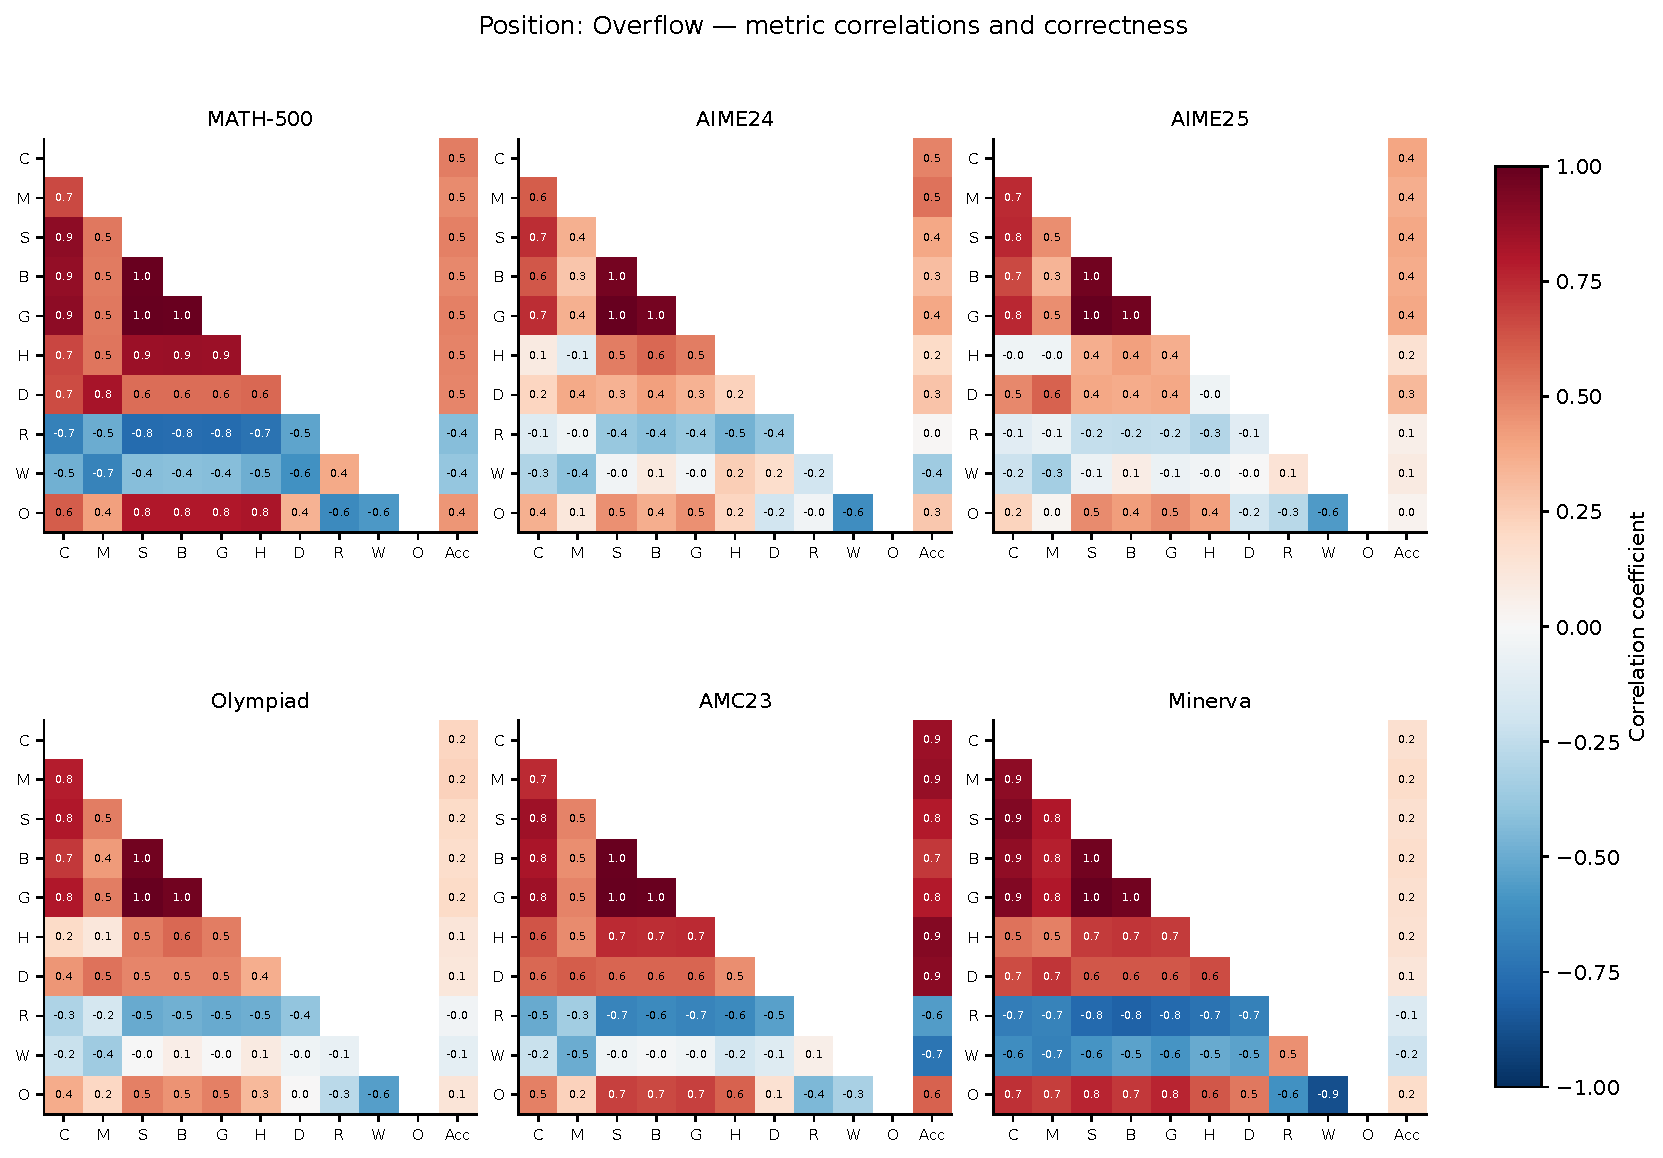
\includegraphics[width=\linewidth]{figures/qwen_atlas_position-overflow.pdf}
\caption{Position: Overflow: metric relationships and correctness. Codes are defined in Table~\ref{tab:qwen-metric-key-atlas}.}
\label{fig:atlas-position-overflow}
\Description{Six benchmark heatmaps compare aggregate metrics with each other and with correctness.}
\end{figure}

\clearpage